\documentclass[12pt]{article}

% Packages
\usepackage{graphicx}
\usepackage{enumerate}
\usepackage{tabularx}
\usepackage{longtable}
\usepackage{booktabs}
\usepackage{caption}

\usepackage{placeins}
\usepackage{float}
\usepackage{multirow}
\captionsetup[table]{skip=2pt}

\usepackage{geometry}                                       
\geometry{left=2.5cm, right=2.5cm, top=2.5cm, bottom=2.5cm} 

\newcounter{TestCounter}
\setcounter{TestCounter}{0}

\newcounter{ResultCounter}
\setcounter{ResultCounter}{0}

\title{
ClinicFlow
\\\vspace{10mm}
\Large \textbf{Test Report}
\vspace{40mm}
}
\author{ Maxim Vasiliev \#400043983
\and
Susie Yu \#000955758
\and
Karl Knopf \#001437217
\and
Weilin Hu \#001150873
\and
Yunfeng Li \#001335650
}
\date{\today}

% Document adapted from https://github.com/studouglas/GEANT4-GPU/blob/master/Documentation/TestPlan/Test%20Plan.tex 
% and http://itq.ch/pdf/Roadmap%20for%20Testing.pdf


\begin{document}
\pagenumbering{gobble}
\maketitle
\newpage
\tableofcontents
\newpage
\pagenumbering{arabic}
\setlength\parindent{0pt}

\section*{List of Tables}

\begin{center}
\begin{tabular}{cl}
\toprule

\bf Table \# & \bf Title\\\midrule

\ref{Table_Acronyms} & Definitions and Acronyms\\
\ref{PatientInput_unit} & Patient Schedule Input Unit Tests \\
\ref{PatientOutput_unit} & Patient Schedule Output Unit Tests \\
\ref{HealthCareInput_unit}& Health Care Scheduling Input Unit Tests\\
\ref{HealthCareOutput_unit}& Health Care Scheduling Output Unit Tests \\
\ref{ClinicModuleInput_unit}& Module Input Unit Tests \\
\ref{ClinicModuleOutput_unit} &Module Output Unit Tests \\
\ref{SimulationEngine_unit} & Simulation Engine Unit Tests \\

\ref{Login_SystemTests} & Login System Tests \\
\ref{DataStorage_SystemTests} & Database Storage System Tests \\
\ref{DataManipulation_SystemTests} & View, Modify and Delete Data System Tests \\
\ref{ScheduleGeneration_SystemTests} & Schedule Generation System Tests \\
\ref{ViewSchedule_SystemTests} & View Schedule and Modify Schedule System Tests \\
\ref{Usability Tests} & Usability Tests \\
\ref{Performance Tests} & Performance Tests \\
\ref{Table_Schedule} & Testing Schedule \\
\bottomrule
\end{tabular}
\end{center}


\section{Introduction}

\subsection{Introduction}

\subsection{Definitions and Terms} 
\begin{center}
\begin{longtable}{>{\raggedright\arraybackslash}p{0.25\textwidth}>{\raggedright\arraybackslash}p{0.65\textwidth}}
\caption{Definitions and Acronyms}\label{Table_Acronyms}\\
\toprule

\bf Term & \bf Definition\\\midrule
Provider & Someone who works in the clinic environment (a nurse, doctor, technician)\\\midrule
Module & A section of the clinic \\ \midrule
Passport & Time record of patients inside the clinic \\ 
\bottomrule
\end{longtable}
\end{center}

\section{Unit Testing}
\subsection{Overview}
	As the programs will be written in the Python 3 programming language, we can use the unittest framework. We will define test cases, with inputs and expected outputs and then be able to run this for each module in the system. 

\subsection{Patient Scheduling: PatientSchedule.py} 
	We have a module in the program that will take in a file containing patients in the clinic, and produce a schedule for them. First we must test if scheduling system can take appropriate inputs. The initial inputs for this test would be that the program has nothing loaded into it currently. First test the class of initializing patient information by collecting data from inputs. This parameter should read the stored information which includes identification and reserved services.

		\subsubsection{Test Inputs}
		\begin{center}
			\begin{longtable}{c>{\raggedright\arraybackslash}p{8.8cm} }
				\caption{Unit Tests - \texttt{Patient Schedule-Input See \ref{patientdateset} }}\label{PatientInput_unit}\\
				\toprule
				\bf Test\# & \bf Inputs \\\midrule
				\refstepcounter{TestCounter}\arabic{TestCounter}
				 & No patient dataset\\
				\\\midrule
				\refstepcounter{TestCounter}\arabic{TestCounter}
				& Sample (valid) patients dataset 
				following the expected inputs format which only contains identification and reserved services  \\
				\\\midrule
				\refstepcounter{TestCounter}\arabic{TestCounter}
				& Sample (valid) patients dataset, but reserved services don't follow the standard sequences
				  \\
				\\\midrule
				\refstepcounter{TestCounter}\arabic{TestCounter}
				& Incorrectly formatted patient dataset, missing the information of reserved service\\
				\bottomrule
			\end{longtable}
		\end{center}
		
		\subsubsection{Test Results}
		\begin{center}
			\begin{longtable}{c>{\raggedright\arraybackslash}p{8.8cm} }
				\caption{Unit Tests - \texttt{Patient Schedule-Input: Results March 2017 See \ref{patientdateset}}}\label{PatientInput_unit_Results}\\
				\toprule
				\bf Test\# & \bf Inputs \\\midrule
				\refstepcounter{ResultCounter}\arabic{ResultCounter}
				& Program crash, error: can't find the patient file\\
				\\\midrule
				\refstepcounter{ResultCounter}\arabic{ResultCounter}
				& Program successfully loads patients information into the system and continues to run.\\
				\\\midrule
				\refstepcounter{ResultCounter}\arabic{ResultCounter}
				& Program successfully loads patients information into the system even the service order doesn't match clinic process
				\\
				\\\midrule
				\refstepcounter{ResultCounter}\arabic{ResultCounter}
				& Program crash, can not read the data from file because of index error\\
				\bottomrule
			\end{longtable}
		\end{center}
		
	
		
	We must also check the function that will output the
	schedule in a usable form for the rest of the system. The results should displays the each patient's identification, scheduled arriving time and reserved services.
	
		\subsubsection{Test Inputs}
		\begin{center}
			\begin{longtable}{c>{\raggedright\arraybackslash}p{8.8cm} }
				\caption{Unit Tests - \texttt{Patient Schedule-Output See \ref{patientschedule}  }}\label{PatientOutput_unit}\\
				\toprule
				\bf Test\# & \bf Inputs \\\midrule
				\refstepcounter{TestCounter}\arabic{TestCounter}
				& Input a 25 sample patients dataset\\
				\\\midrule
				\refstepcounter{TestCounter}\arabic{TestCounter}
				& Input a 40 sample patients dataset  \\
				\\\midrule
				\refstepcounter{TestCounter}\arabic{TestCounter}
				& Input a dataset while patient's services not in order\\
				\bottomrule
			\end{longtable}
		\end{center}
		
		\subsubsection{Test Results}
		\begin{center}
			\begin{longtable}{c>{\raggedright\arraybackslash}p{8.8cm} }
				\caption{Unit Tests - \texttt{Patient Schedule-Output : Results March 2017 See \ref{patientschedule} }}\label{PatientOutput_unit_results}\\
				\toprule
				\bf Test\# & \bf Inputs \\\midrule
				\refstepcounter{ResultCounter}\arabic{ResultCounter}
				& Program successfully generates schedules for each patient based on inputs.
				The output is a usable form\\
				\\\midrule
				\refstepcounter{ResultCounter}\arabic{ResultCounter}
				& Program successfully generates schedules for each patient,
				but it assigned patients schedule time after clinic open hour.
				The output is usable form with errors  \\
				\\\midrule
				\refstepcounter{ResultCounter}\arabic{ResultCounter}
				& Program successfully generates schedules for each patient,
				even the services don't follow the clinic process. The output is not a usable form  \\
				\bottomrule
			\end{longtable}
		\end{center}
	
	
		
\subsection{Healthcare Worker Scheduling: HealthCareSchedule.py} 
We have a module in the program that will take in a file containing the names and break schedule of the providers. It will then generate a schedule object that the simulation can use.
		\subsubsection{Test Inputs}
		\begin{center}
			\begin{longtable}{c>{\raggedright\arraybackslash}p{8.8cm} }
				\caption{Unit Tests - \texttt{HealthCare Schedule-Input See \ref{healthworkerset} }}\label{HealthCareInput_unit}\\
				\toprule
				\bf Test\# & \bf Inputs \\\midrule
				\refstepcounter{TestCounter}\arabic{TestCounter}
				& No health care worker dataset\\
				\\\midrule
				\refstepcounter{TestCounter}\arabic{TestCounter}
				& Sample (valid) healthcare worker dataset following the expected format which contains worker's identification, break schedule sets and clinic sections for the worker to dealing with\\
				\\\midrule
				\refstepcounter{TestCounter}\arabic{TestCounter}
				& Incorrectly formated healthcare worker dataset which doesn't have breaking time or in charged duty\\
				\bottomrule
			\end{longtable}
		\end{center}
	
		\subsubsection{Test Results}
		\begin{center}
			\begin{longtable}{c>{\raggedright\arraybackslash}p{8.8cm} }
				\caption{Unit Tests - \texttt{Health Care Schedule-Results April 2017 See \ref{healthworkerset} }}\label{HealthCareInput_unit_results}\\
				\toprule
				\bf Test\# & \bf Inputs \\\midrule
				\refstepcounter{ResultCounter}\arabic{ResultCounter}
				& Program crash, error: can not find the health care file\\
				\\\midrule
				\refstepcounter{ResultCounter}\arabic{ResultCounter}
				& Program successfully loads and stores the information of clinic workers and continue to run\\
				\\\midrule
				\refstepcounter{ResultCounter}\arabic{ResultCounter}
				& Program crash, can not read data from file \\
				\bottomrule
			\end{longtable}
		\end{center}
	
	
		We must also check the function that will output the
		schedule in a usable form for the rest of the system.
		
			\subsubsection{Test Inputs}
			\begin{center}
				\begin{longtable}{c>{\raggedright\arraybackslash}p{8.8cm} }
					\caption{Unit Tests - \texttt{Health Care Schedule-Output See \ref{healthworkerset} }}\label{HealthCareOutput_unit}\\
					\toprule
					\bf Test\# & \bf Inputs \\\midrule
					\refstepcounter{TestCounter}\arabic{TestCounter}
					& Input 6 workers and their break time schedules. Each worker is dealing with one service of the clinic. Input 1 worker who is flexible for all services with break time schedule\\
					\\\midrule
					\refstepcounter{TestCounter}\arabic{TestCounter}
					& Input 4 worker and their break time schedules with improper value. Each worker is dealing with one service of the clinic. \\
					\bottomrule
				\end{longtable}
			\end{center}
			
			\subsubsection{Test Results}
			\begin{center}
				\begin{longtable}{c>{\raggedright\arraybackslash}p{8.8cm} }
					\caption{Unit Tests - \texttt{HealthCare-Output : Results April 2017 See \ref{healthworkerset} }}\label{HealthCareOutput_unit_results}\\
					\toprule
					\bf Test\# & \bf Inputs \\\midrule
					\refstepcounter{ResultCounter}\arabic{ResultCounter}
					& Program successfully loads and stores the information of clinic workers include the break time sets and responsibilities. The output is usable\\
					\\\midrule
					\refstepcounter{ResultCounter}\arabic{ResultCounter}
					& Program successfully loads and stores the data of clinic workers with improper values, which can cause no break, too many breaks and no service available. The output is in a usable form with errors   \\
					\bottomrule
				\end{longtable}
			\end{center}
		

\subsection{Clinic: Clinic.py} 
Clinics can have a variety of sections (which we shall call modules)  such as Blood taking or xray. Each section can be unique or have multiples. We model each clinic in a data file, which will be read into the system when a simulation is run for that clinic.
		
		\subsubsection{Test Inputs}
		\begin{center}
			\begin{longtable}{c>{\raggedright\arraybackslash}p{8.8cm} }
				\caption{Unit Tests - \texttt{Clinic Modules-Input See \ref{moduledataset} }}\label{ClinicModuleInput_unit}\\
				\toprule
				\bf Test\# & \bf Inputs \\\midrule
				\refstepcounter{TestCounter}\arabic{TestCounter}
				& No clinic module dataset\\
				\\\midrule
				\refstepcounter{TestCounter}\arabic{TestCounter}
				& Sample (valid) module dataset with the expected format which contains module name, prerequest module, maximum capacity of worker, minimum capacity of worker, average service time and service time variance\\
				\\\midrule
				\refstepcounter{TestCounter}\arabic{TestCounter}
				& Incorrectly formated healthcare worker dataset which missing some information\\
				\bottomrule
			\end{longtable}
		\end{center}
		
		\subsubsection{Test Results}
		\begin{center}
			\begin{longtable}{c>{\raggedright\arraybackslash}p{8.8cm} }
				\caption{Unit Tests - \texttt{ClinicModuleInput-Results April 2017 See \ref{moduledataset}}}\label{ClinicModuleInput_unit_results}\\
				\toprule
				\bf Test\# & \bf Inputs \\\midrule
				\refstepcounter{ResultCounter}\arabic{ResultCounter}
				& Program crash, error: can not find the module file\\
				\\\midrule
				\refstepcounter{ResultCounter}\arabic{ResultCounter}
				& Program successfully loads and stores the information of clinic modules and continue to run\\
				\\\midrule
				\refstepcounter{ResultCounter}\arabic{ResultCounter}
				& Program crash, can not read data from file \\
				\bottomrule
			\end{longtable}
		\end{center}
	
	
We must also check that the functions in this module create a valid network of modules for the clinic. 
		
		\subsubsection{Test Inputs}
		\begin{center}
			\begin{longtable}{c>{\raggedright\arraybackslash}p{8.8cm} }
				\caption{Unit Tests - \texttt{Clinic Module-Output See \ref{moduledataset}}}\label{ClinicModuleOutput_unit}\\
					\toprule
					\bf Test\# & \bf Inputs \\\midrule
					\refstepcounter{TestCounter}\arabic{TestCounter}
					& Input data of the 6 modules of the clinic(Register, RNInterview, ECG, Bloodwork, Anesthesiologist, X-ray)\\
					\\\midrule
					\refstepcounter{TestCounter}\arabic{TestCounter}
					& Input duplicate the modules \\
					\bottomrule
				\end{longtable}
			\end{center}
			
		\subsubsection{Test Results}
		\begin{center}
			\begin{longtable}{c>{\raggedright\arraybackslash}p{8.8cm} }
				\caption{Unit Tests - \texttt{ClinicModule-Output : Results April 2017 See \ref{moduledataset}}}\label{ClinicModuleOutput_unit_results}\\
				\toprule
				\bf Test\# & \bf Inputs \\\midrule
				\refstepcounter{ResultCounter}\arabic{ResultCounter}
				& Program successfully loads and stores the data of clinic modules. The output is usable\\
				\\\midrule
				\refstepcounter{ResultCounter}\arabic{ResultCounter}
				& Program successfully loads and stores the data of clinic workers with duplicates. The output is in a usable form  \\
				\bottomrule
			\end{longtable}
		\end{center}
	
We have analysis for  the clinic passport data and evaluate the average processing time 
as well as the processing time variance in each module. 

	\subsubsection{Test Inputs}
	\begin{center}
		\begin{longtable}{c>{\raggedright\arraybackslash}p{8.8cm} }
			\caption{Unit Tests - \texttt{Clinic Modules Data Analysis-Input See \ref{passportcreate} }}\label{ClinicAnalysisInput_unit}\\
			\toprule
			\bf Test\# & \bf Inputs \\\midrule
			\refstepcounter{TestCounter}\arabic{TestCounter}
			& No clinic passport dataset\\
			\\\midrule
			\refstepcounter{TestCounter}\arabic{TestCounter}
			& Sample (refined) passport data of clinic over period of time which contains schedule time, arriving time, departing time, start and over time in each module\\
			\\\midrule
			\refstepcounter{TestCounter}\arabic{TestCounter}
			& Unrefined passport data \\
			\bottomrule
		\end{longtable}
	\end{center}
	
	\subsubsection{Test Results}
	\begin{center}
		\begin{longtable}{c>{\raggedright\arraybackslash}p{8.8cm} }
			\caption{Unit Tests - \texttt{Clinic Modules Data Analysis-Input-Results April 2017 See \ref{passportcreate}}}\label{ClinicAnalysisInput_unit_results}\\
			\toprule
			\bf Test\# & \bf Inputs \\\midrule
			\refstepcounter{ResultCounter}\arabic{ResultCounter}
			& Program crash, error: can not find the passport file\\
			\\\midrule
			\refstepcounter{ResultCounter}\arabic{ResultCounter}
			& Program successfully loads and stores the information of clinic modules and continue to run\\
			\\\midrule
			\refstepcounter{ResultCounter}\arabic{ResultCounter}
			& Program crash, can't read data from file \\
			\bottomrule
		\end{longtable}
	\end{center}
	
We must also check the function that will output the
data analysis of passport(the tiem records of patients inside clinic) 
in a usable form for the rest of the system.
	
	\subsubsection{Test Inputs}
	\begin{center}
		\begin{longtable}{c>{\raggedright\arraybackslash}p{8.8cm} }
			\caption{Unit Tests - \texttt{Clinic Modules Data Analysis-Output See \ref{passportcreate}}}\label{ClinicAnalysisOutput_unit}\\
			\toprule
			\bf Test\# & \bf Inputs \\\midrule
			\refstepcounter{TestCounter}\arabic{TestCounter}
			& Full data of refined passport file\\
			\\\midrule
			\refstepcounter{TestCounter}\arabic{TestCounter}
			& Half data of refined passport file \\
			\bottomrule
		\end{longtable}
	\end{center}
	
	\subsubsection{Test Results}
	\begin{center}
		\begin{longtable}{c>{\raggedright\arraybackslash}p{8.8cm} }
			\caption{Unit Tests - \texttt{Clinic Modules Data Analysis-Output : Results April 2017 See \ref{passportcreate}}}\label{ClinicAnalysisOutput_unit_results}\\
			\toprule
			\bf Test\# & \bf Inputs \\\midrule
			\refstepcounter{ResultCounter}\arabic{ResultCounter}
			& Data analysis successfully generates the module file based on passport file. The output is usable\\
			\\\midrule
			\refstepcounter{ResultCounter}\arabic{ResultCounter}
			& Data analysis successfully generates the module file based on passport file. The output is usable\\
			\bottomrule
		\end{longtable}
	\end{center}

\subsection{Simulation Engine: SimulationEngine.py} 
The system relies on the simulation engine to generate any results. This module must be able to take in the previous schedules and data, and use that to run a discrete event simulation using those schedules. The pass criteria for this engine should be that it is capable of generating realistic schedules. To do this, we ran data set through the engine and randomly selected patients to check to see if they followed a logical path through the clinic.
	
	
	\subsubsection{Test Inputs}
	\begin{center}
		\begin{longtable}{c>{\raggedright\arraybackslash}p{8.8cm} }
			\caption{Unit Tests - \texttt{Simulation Engine See \ref{simulationtests} }}\label{SimulationEngine_unit}\\
			\toprule
			\bf Test\# & \bf Inputs \\\midrule
			\refstepcounter{TestCounter}\arabic{TestCounter}
			& A passport dataset based on actual clinic data, 25 sample patients, 
			6 health workers each deals with one of the clinic service, 
			1 health worker is flexible with all services, all workers have different break time schedule \\
			\\\midrule
			\refstepcounter{TestCounter}\arabic{TestCounter}
			& A passport dataset based on actual clinic data, 50 sample patients, 
			6 health workers each deals with one of the clinic service, 
			1 health worker is flexible with all services, all workers have different break time schedule \\
			\\\midrule
			\refstepcounter{TestCounter}\arabic{TestCounter}
			& A passport dataset based on actual clinic data, 19 sample patients, 
			2 health workers are flexible with all services, all workers have different break time schedule \\
			\\\midrule
			\refstepcounter{TestCounter}\arabic{TestCounter}
			& A passport dataset based on actual clinic data, 19 sample patients, 
			6 health workers each deals with one of the clinic service, 
			1 health worker is flexible with all services, all workers have same break time schedule \\
			\\\midrule
			\refstepcounter{TestCounter}\arabic{TestCounter}
			& A clinic dataset not based on actual clinic data, 19 sample patients, 
			6 health workers each deals with one of the clinic service, 
			1 health worker is flexible with all services, all workers have same break time schedule \\
			\bottomrule
		\end{longtable}
	\end{center}

\subsubsection{Test Results}
\begin{center}
	\begin{longtable}{c>{\raggedright\arraybackslash}p{8.8cm} }
		\caption{Unit Tests - \texttt{Simulation Engine : Results April 2017 See \ref{simulationtests}}}\label{SimulationEngine_unit_results}\\
		\toprule
		\bf Test\# & \bf Inputs \\\midrule
		\refstepcounter{ResultCounter}\arabic{ResultCounter}
		& Simulation engine successfully load data from passport dataset, patient dataset and heath worker dataset. Based on given data, simulation engine successfully simulate the time line of patients inside clinic. The simulated processing time of each clinic module is consider as too short\\
		\\\midrule
		\refstepcounter{ResultCounter}\arabic{ResultCounter}
		& Simulation engine successfully generate results. Since the large number of patients, not all patients can finish before clinic close\\
		\\\midrule
		\refstepcounter{ResultCounter}\arabic{ResultCounter}
		& Simulation engine successfully generate results. It turns out that the mechanism for flexible health workers doesn't work properly. The worker won't change clinic module until break which cause many modules become unavailable to work. Patients don't follow the order of process.\\
		\\\midrule
		\refstepcounter{ResultCounter}\arabic{ResultCounter}
		& Simulation engine successfully generate results. When all workers take break at same time, all services stop. \\
		\\\midrule
		\refstepcounter{ResultCounter}\arabic{ResultCounter}
		& Simulation engine successfully generate results. With the manually input large average module processing time, the processing time of simulation is still consider as too short\\
		\bottomrule
	\end{longtable}
\end{center}




\section{System Testing}
\subsection{Login} 
The purpose of user login is to ensure that only valid users allowed to in access the system. There are two types of account. One is the  administrator account which has full authority to manipulate the data and control all operable functions of the system. Another one is the viewer account which only can view the information.  Testing retrieves the input account and password and match with the account information in an existing database to determine whether the user is valid and what the user can do.
\begin{center}
\begin{longtable}{c>{\raggedright\arraybackslash}p{4.8cm} >{\raggedright\arraybackslash}p{3cm}>{\raggedright\arraybackslash}p{3cm}}
\caption{System Tests: Login}\label{Login_SystemTests}\\
\toprule
\bf \# & \bf Initial State & \bf Inputs & \bf Pass Criteria\\\midrule
\stepcounter{TestCounter}\arabic{TestCounter} 
& Login Page
Empty input field of account and password.
& Empty input of one of the input fields or both. Click login.
& Stay at same page and error message of empty input.
\\\midrule
\stepcounter{TestCounter}\arabic{TestCounter} 
& Login Page
Empty input field of account and password.
& Valid input of account and password of administrator account. Click login.
& Redirect to the main page of the application, and give user full authority of control.
\\\midrule
\stepcounter{TestCounter}\arabic{TestCounter} 
&Login Page
Empty input field of account and password.
& Valid input of account and password of viewer account .
Click login.
& Redirect to the main page of the application, user only allowed to view the data and schedule.
\\\midrule
\stepcounter{TestCounter}\arabic{TestCounter} 
&Login Page
Empty input field of account and password.
& Invalid of account or invalid password.
Click login.
& Stay at the same page and present an error message of the invalid login.
\\\midrule
\stepcounter{TestCounter}\arabic{TestCounter} 
&Application main page
& Click logout.
& Redirect to the login page.
\\\midrule
\bottomrule
\end{longtable}
\end{center}
\subsection{Insertion and Storage of Data} 
The application should allow administrator account user to insert data such as patient procedure, doctor and nurse shift hours and other necessary data into corresponding databases. The testing will compare the inserted data with the data stored in database. There exists a checking module to validate the input values.
\begin{center}
	\begin{longtable}{c>{\raggedright\arraybackslash}p{4.8cm} >{\raggedright\arraybackslash}p{3cm}>{\raggedright\arraybackslash}p{3cm}}
		\caption{System Tests: Data Storage}\label{DataStorage_SystemTests}\\
		\toprule
		\bf \# & \bf Initial State & \bf Inputs & \bf Pass Criteria \\\midrule
		\stepcounter{TestCounter}\arabic{TestCounter} 
		& Application main page, admin account.
		& Click Add Data.
		& Redirect to the Application adding data page.
		\\\midrule
		\stepcounter{TestCounter}\arabic{TestCounter} 
		& Application adding data page.
		& Add the inexistent data to target database with correct data type. Click submit.
		& Stay in same page and all inputs are cleaned. Data appear in the corresponding database.
		\\\midrule
		\stepcounter{TestCounter}\arabic{TestCounter} 
		& Application adding data page.
		& Add the data to target database with incorrect data type or incorrect pattern.
		Click submit.
		& Stay in same page and save valid data. Error messages indicate the invalid inputs.
		\\\midrule
		\stepcounter{TestCounter}\arabic{TestCounter} 
		& Application adding data page.
		& Add the data which already existed in target database. Click submit.
		& Stay in same page and save data. Error message indicates the redundancy of data.
		\\\midrule
		\stepcounter{TestCounter}\arabic{TestCounter} 
		& Application adding data page.
		& Add data which out of domain (such as reservation date in past days) to target database. Click submit.
		& Stay in same page and save data. Error message indicates that the data out of valid range.
		\\\midrule
		\stepcounter{TestCounter}\arabic{TestCounter} 
		& Application main page, viewer account.
		& Click Add Data. 
		& Error message.
		\\\midrule
		\bottomrule
	\end{longtable}
\end{center}
\subsection{View, Modify and Delete Data} 
Administrator account user can view, modify and delete existed data in database. Viewer account user only can read the data in the database.  According to the selection of user, retrieve corresponding database and display the content on user interface. Changes and deletion created by administrator account user should be stored into database. Testing checks whether the application display right data, and  whether the changes synchronize with database. Test the validation of the database when unexpected actions happen.
\begin{center}
	\begin{longtable}{c>{\raggedright\arraybackslash}p{4.8cm} >{\raggedright\arraybackslash}p{3cm}>{\raggedright\arraybackslash}p{3cm}}
		\caption{System Tests: Data Manipulation}\label{DataManipulation_SystemTests}\\
		\toprule
		\bf \# & \bf Initial State & \bf Inputs & \bf Pass Criteria \\\midrule
		\stepcounter{TestCounter}\arabic{TestCounter} 
		& Application main page, admin and viewer account .
		& Click View Data.
		& Redirect to the View Data page.
		\\\midrule
		\stepcounter{TestCounter}\arabic{TestCounter} 
		& Application view data page, admin and viewer account.
		& Select target database, click view.
		& Stay at same page. Display the content of all data from corresponding database.
		\\\midrule
		\stepcounter{TestCounter}\arabic{TestCounter} 
		& Application view data page, admin and view account.
		& Select target database and give specific condition, click view. 
		& Stay at same page. Display the content of target data from corresponding database.
		\\\midrule
		\stepcounter{TestCounter}\arabic{TestCounter} 
		& Application view data page, admin account.
		& Modify the displayed data and change the value by another valid value. Click save.
		& Stay at same page. The value in display area and database have been changed.
		\\\midrule
		\stepcounter{TestCounter}\arabic{TestCounter} 
		& Application view data page, admin account.
		& Modify the displayed data and change the value by invalid value( empty for required value or out of valid range). Click save.
		& Stay at same page, no change happen in displayed data or database. Error messages indicate the unexpected changes.
		\\\midrule
		\stepcounter{TestCounter}\arabic{TestCounter} 
		& Application view data page, admin account.
		& Delete whole one row of data by clicking deletion button at end of the row. Click save. 
		& Stay at same page. The deleted row disappear and the data in database is deleted as well.
		\\\midrule
		\stepcounter{TestCounter}\arabic{TestCounter} 
		& Application view data page, admin account.
		& Delete whole one row of data if the data is expected to use in future (Patient reservation in next few days). Click save.
		& Stay at same page. Pop up a deletion confirmation window. Confirming  the deletion will remove the row from the list. Cancel deletion will save the data.
		\\\midrule
		\stepcounter{TestCounter}\arabic{TestCounter} 
		& Application view data page, viewer account.
		& Modify the displayed data. 
		& Stay at same page. Data is not editable.
		\\\midrule
		\stepcounter{TestCounter}\arabic{TestCounter} 
		& Application view data page, viewer account.
		& Click delete button.
		& Stay at same page. Deletion button does not exist.
		\\\midrule
		\stepcounter{TestCounter}\arabic{TestCounter} 
		& Application view data page, viewer account.
		& Click save.
		& Stay at same page.
		Save button does not exist .
		\\\midrule		
		\bottomrule
	\end{longtable}
\end{center}
\subsection{Schedule Generation} 
The application retrieves data from databases and generates schedules based on back end algorithms. Generating schedule is a critical part in the application, because the Clinic needs accurate schedules without conflicts to maintain the efficiency and minimize the wasting of time for both parties. Thus the generated schedule should be examined carefully by the users. 
\begin{center}
	\begin{longtable}{c>{\raggedright\arraybackslash}p{4.8cm} >{\raggedright\arraybackslash}p{3cm}>{\raggedright\arraybackslash}p{3cm}}
		\caption{System Tests: Schedule Generation}\label{ScheduleGeneration_SystemTests}\\
		\toprule
		\bf \# & \bf Initial State & \bf Inputs & \bf Pass Criteria \\\midrule
		\stepcounter{TestCounter}\arabic{TestCounter} 
		& Application main page, admin account
		& Click generate schedule
		& Redirect to generate page schedule
		\\\midrule
		\stepcounter{TestCounter}\arabic{TestCounter} 
		& Application generate schedule page 
		& Select the type of schedule, click start generating.
		& Create a schedule and display it to user. Saved the schedule into corresponding database.
		\\\midrule
		\stepcounter{TestCounter}\arabic{TestCounter} 
		& Application generate schedule page
		& Insert several data of patients reserve same day, same time, different clinic slots. Select the type of schedule, click start generating.
		& Create a schedule and display it to user. The patients can be issued to same time. Saved the schedule into corresponding database.
		\\\midrule
		\stepcounter{TestCounter}\arabic{TestCounter} 
		& Application generate schedule page
		& Insert several data of patients reserve same day, same time, same clinic slots. Select the type of schedule, click start generating.
		& Create a schedule and display it to user. The patients should be spreaded to different time periods. Saved the schedule into corresponding database.
		\\\midrule
		\stepcounter{TestCounter}\arabic{TestCounter} 
		& Application main page, view account
		& Click generate schedule
		& Stay at same page.
		Generate schedule does not exist.
		\\\midrule
		\bottomrule
	\end{longtable}
\end{center}

\subsection{View Schedule and Modify Schedule}
The application allows administrator account user and viewer account user to view the generated schedules. Administrator account user also has the permission to adjust the schedule. Testing ensures that the changed schedule doesn’t have conflicts. 
\begin{center}
	\begin{longtable}{c>{\raggedright\arraybackslash}p{4.8cm} >{\raggedright\arraybackslash}p{3cm}>{\raggedright\arraybackslash}p{3cm}}
		\caption{System Tests: View Schedule and Modify Schedule}\label{ViewSchedule_SystemTests}\\
		\toprule
		\bf \# & \bf Initial State & \bf Inputs & \bf Pass Criteria \\\midrule
		\stepcounter{TestCounter}\arabic{TestCounter} 
		& Application main page, admin and viewer account.
		& Click view schedule. 
		& Redirect to the view schedule page.
		\\\midrule
		\stepcounter{TestCounter}\arabic{TestCounter} 
		& Application view schedule page, admin and viewer account.
		& Select type and date of the schedule. Click view.
		& Stay at same page. The page displays the existed schedule.
		\\\midrule
		\stepcounter{TestCounter}\arabic{TestCounter} 
		& Application view schedule page, admin account.
		& Click adding button and add a new reserved time into blank area of schedule. Click save.
		& Stay at same page. The new time period is added into schedule.The new schedule is saved into database.
		\\\midrule
		\stepcounter{TestCounter}\arabic{TestCounter} 
		& Application view schedule, page admin account.
		& Click on adding button on a reserved area. Click save 
		& If no error happens , stay at same page. No adding button on a reserved area.
		\\\midrule
		\stepcounter{TestCounter}\arabic{TestCounter} 
		& Application view schedule page, admin account 
		& Click on moving button on a reserved area and choose an empty area. Click save.
		& If no error happens stay at same page. The selected time period is set at new area. The new schedule is saved into database.
		\\\midrule
		\stepcounter{TestCounter}\arabic{TestCounter} 
		& Application view schedule page, admin account 
		& Click on moving button on a reserved area and choose a reserved area. Switch the reservation. Click save.
		& If no error happens, stay at same page. The selected time period  is switched with another one. The new schedule is saved into database.
		\\\midrule
		\stepcounter{TestCounter}\arabic{TestCounter} 
		& Application view schedule page, admin account.
		& Application validates the changes of schedule.
		& Checks on the sequences of procedures in clinic. If adding, moving, and switching violate the the sequence, show error message.
		\\\midrule
		\stepcounter{TestCounter}\arabic{TestCounter} 
		& Application view schedule page, admin account.
		& Click delete button to remove a reservation. Click save. 
		& Pop up a window for deletion confirmation. If continue to delete, remove the reservation. Save the new schedule to database. 
		\\\midrule
		\stepcounter{TestCounter}\arabic{TestCounter} 
		& Application view schedule page, viewer account.
		& Click adding or  click moving or click delete or click save.
		& Stay at same page. No adding button, no moving button, no deletion button, no save button.
		\\\midrule
		\bottomrule
	\end{longtable}
\end{center}


\section{Non-Functional Requirements Testing}

\subsection{Usability}
\begin{center}
	\begin{longtable}{c>{\raggedright\arraybackslash}p{4.8cm} >{\raggedright\arraybackslash}p{3.5cm}>{\raggedright\arraybackslash}p{3cm}>{\raggedright\arraybackslash}p{3cm}}
		\caption{Usability Tests}\label{Usability Tests}\\
		\toprule
		\bf \# & \bf Description & \bf Type & \bf Criterion & Tester(s) \\\midrule
		\stepcounter{TestCounter}\arabic{TestCounter} 
		& We will list the most frequently performed tasks, and the development
		team will use the product to complete them. We count the number of
		mouse clicks.
		& Functional (dynamic, manual)	
		& The average number of mouse clicks should be less than five.    
		& 	Development Team
		\\\midrule
		\stepcounter{TestCounter}\arabic{TestCounter} 
		& We will invite five doctors and five nurses to use our product and
		give them a three minutes demonstration on how to complete a certain
		task. After that, the participants will try to complete the same task.
		& Functional (dynamic, manual)	
		& The participants can complete the same task correctly in three minutes.  
		& 	Testing Team
		\\\midrule
		\stepcounter{TestCounter}\arabic{TestCounter} 
		& We will invite five doctors and five nurses to use our product, but
		we will not give a demonstration on how to complete a certain task.
		Instead, the participants will try to complete it based
		on their previous experience and the hints provided by the application.
		& Functional (dynamic, manual)	
		& The participants can complete the required tasks in five minutes and
		they should encounter fewer than three errors.  
		& 	Testing Team
		\\\midrule
		\bottomrule
	\end{longtable}
\end{center}

\subsection{Performance Testing}
\begin{center}
	\begin{longtable}{c>{\raggedright\arraybackslash}p{4.8cm} >{\raggedright\arraybackslash}p{3.5cm}>{\raggedright\arraybackslash}p{3cm}>{\raggedright\arraybackslash}p{3cm}}
		\caption{Performance Tests}\label{Performance Tests}\\
		\toprule
		\bf \# & \bf Description & \bf Type & \bf Criterion & Tester(s) \\\midrule
		\stepcounter{TestCounter}\arabic{TestCounter} 
		& The development team will use the product to complete the most frequently performed tasks.
		We will calculate the time from the start-up of the application to the completion of the work.
		& Functional (dynamic, manual)	
		& The average time should be less than five minutes.  
		& 	Development Team
		\\\midrule
		\stepcounter{TestCounter}\arabic{TestCounter} 
		& The development team will generate 100000 data points, which is ten times more
		than the expected data points. We will input those data points into our
		application. Next, we will input 100 times more data points into the application.
		& Functional (dynamic, manual)	
		& The application does not crash, and there are no obvious latencies
		(less than 5 seconds for each task) when performing
		the common tasks in the first case. The application can crash in the second case.  
		& 	Development Team
		\\\midrule
		\stepcounter{TestCounter}\arabic{TestCounter} 
		& The development team will generate random data points, which contain problems such as
		incorrect formatting data and illegal characters. We will input those data points into
		our application.
		& Functional (dynamic, manual)	
		& The application does not crash and prompts the users that the input data is not
		correct and how they could correct it.  
		& 	Development Team
		\\\midrule
		\bottomrule
	\end{longtable}
\end{center}

%\section{Automated Testing}

%\subsection{Automated System Testing}

%\subsection{Automated Unit Testing}


\newpage
\section{Collected Samples}
\subsection{Patient Dataset Test} \label{patientdateset}
	\subsubsection{Expected formated inputs}
	\begin{verbatim}
	Patient1 Registration,RNInterview,LaboratoryECG,LaboratoryBloodwork,
	Anesthesiologist,XrayinRadiology
	
	Patient2 Registration,RNInterview,LaboratoryECG,LaboratoryBloodwork,
	Anesthesiologist,XrayinRadiology
	
	Patient3 Registration,RNInterview,LaboratoryECG,LaboratoryBloodwork,
	Anesthesiologist,XrayinRadiology
	
	Patient4 Registration,RNInterview,LaboratoryECG,LaboratoryBloodwork,
	Anesthesiologist
	
	Patient5 Registration,RNInterview,LaboratoryECG,LaboratoryBloodwork,
	Anesthesiologist,XrayinRadiology
	
	Patient6 Registration,RNInterview,LaboratoryECG,LaboratoryBloodwork
	\end{verbatim}
	\subsubsection{Outputs}
	\begin{verbatim}
	name: Patient1 initial scheduled time: 0 initial arrival time: 0 
	initial station: ['Registration', 'RNInterview', 'LaboratoryECG',
	 'LaboratoryBloodwork', 'Anesthesiologist', 'XrayinRadiology'] 
	 initial location: ['Registration', 'RNInterview', 'LaboratoryECG', 
	 'LaboratoryBloodwork','Anesthesiologist', 'XrayinRadiology']
	  initial completion time: -1 initial service time: 0
	
	name: Patient2 initial scheduled time: 0 initial arrival time: 0 
	initial station: ['Registration', 'RNInterview', 'LaboratoryECG',
	 'LaboratoryBloodwork', 'Anesthesiologist', 'XrayinRadiology'] 
	 initial location: ['Registration', 'RNInterview', 'LaboratoryECG',
	  'LaboratoryBloodwork', 'Anesthesiologist', 'XrayinRadiology'] 
	  initial completion time: -1 initial service time: 0
	
	name: Patient3 initial scheduled time: 0 initial arrival time: 0 
	initial station: ['Registration', 'RNInterview', 'LaboratoryECG',
	 'LaboratoryBloodwork', 'Anesthesiologist', 'XrayinRadiology'] 
	 initial location: ['Registration', 'RNInterview', 'LaboratoryECG', 
	 'LaboratoryBloodwork', 'Anesthesiologist', 'XrayinRadiology']
	  initial completion time: -1 initial service time: 0

	name: Patient4 initial scheduled time: 0 initial arrival time: 0
	 initial station: ['Registration', 'RNInterview', 'LaboratoryECG',
	  'LaboratoryBloodwork', 'Anesthesiologist']
	   initial location: ['Registration', 'RNInterview', 'LaboratoryECG',
	    'LaboratoryBloodwork', 'Anesthesiologist']
	     initial completion time: -1 initial service time: 0

	name: Patient5 initial scheduled time: 0 initial arrival time: 0 
	initial station: ['Registration', 'RNInterview', 'LaboratoryECG',
	 'LaboratoryBloodwork', 'Anesthesiologist', 'XrayinRadiology'] 
	 initial location: ['Registration', 'RNInterview', 'LaboratoryECG',
	  'LaboratoryBloodwork', 'Anesthesiologist', 'XrayinRadiology'] 
	  initial completion time: -1 initial service time: 0

	name: Patient6 initial scheduled time: 0 initial arrival time: 0 
	initial station: ['Registration', 'RNInterview', 'LaboratoryECG', 
	'LaboratoryBloodwork'] initial location: ['Registration', 'RNInterview',
	 'LaboratoryECG', 'LaboratoryBloodwork'] 
	 initial completion time: -1 initial service time: 0
	
	\end{verbatim}
	
\subsection{Patient Schedule Test} \label{patientschedule}
\subsubsection{Expected formated inputs}
	\begin{verbatim}
	Patient1 Registration,RNInterview,LaboratoryECG,LaboratoryBloodwork,
	Anesthesiologist,XrayinRadiology
	Patient2 Registration,RNInterview,LaboratoryECG,LaboratoryBloodwork,
	Anesthesiologist,XrayinRadiology
	Patient3 Registration,RNInterview,LaboratoryECG,LaboratoryBloodwork,
	Anesthesiologist,XrayinRadiology
	Patient4 Registration,RNInterview,LaboratoryECG,LaboratoryBloodwork,
	Anesthesiologist
	Patient5 Registration,RNInterview,LaboratoryECG,LaboratoryBloodwork,
	Anesthesiologist,XrayinRadiology
	Patient6 Registration,RNInterview,LaboratoryECG,LaboratoryBloodwork
	Patient7 Registration,RNInterview,LaboratoryECG,LaboratoryBloodwork,
	Anesthesiologist,XrayinRadiology
	Patient8 Registration,RNInterview,LaboratoryECG,LaboratoryBloodwork,
	Anesthesiologist,XrayinRadiology
	Patient9 Registration,RNInterview,LaboratoryECG,LaboratoryBloodwork,
	Anesthesiologist,XrayinRadiology
	Patient10 Registration,RNInterview,LaboratoryECG,LaboratoryBloodwork
	Patient11 Registration,RNInterview,LaboratoryECG,LaboratoryBloodwork,
	Anesthesiologist,XrayinRadiology
	Patient12 Registration,RNInterview,LaboratoryECG,LaboratoryBloodwork,
	Anesthesiologist
	Patient13 Registration,RNInterview,LaboratoryECG,LaboratoryBloodwork,
	Anesthesiologist,XrayinRadiology
	Patient14 Registration,RNInterview,LaboratoryECG,LaboratoryBloodwork,
	Anesthesiologist,XrayinRadiology
	Patient15 Registration,RNInterview,LaboratoryECG,LaboratoryBloodwork,
	Anesthesiologist,XrayinRadiology
	Patient16 Registration,RNInterview,LaboratoryECG,LaboratoryBloodwork
	Patient17 Registration,RNInterview,LaboratoryECG,LaboratoryBloodwork
	Patient18 Registration,RNInterview,LaboratoryECG,LaboratoryBloodwork
	Patient19 Registration,RNInterview,LaboratoryECG,LaboratoryBloodwork,
	XrayinRadiology
	Patient20 Registration,RNInterview,LaboratoryECG,LaboratoryBloodwork
	Patient21 Registration,RNInterview,LaboratoryECG,LaboratoryBloodwork,
	XrayinRadiology
	Patient22 Registration,RNInterview,LaboratoryECG,LaboratoryBloodwork
	Patient23 Registration,RNInterview,LaboratoryECG,LaboratoryBloodwork,
	XrayinRadiology
	Patient24 Registration,RNInterview,LaboratoryECG,LaboratoryBloodwork
	Patient25 Registration,RNInterview,LaboratoryECG,LaboratoryBloodwork,
	XrayinRadiology
	\end{verbatim}
	
		\subsubsection{Outputs}
		\begin{verbatim}
		Patient1 8:19 ['Registration', 'RNInterview', 'LaboratoryECG',
		 'LaboratoryBloodwork', 'Anesthesiologist', 'XrayinRadiology']
		Patient2 8:36 ['Registration', 'RNInterview', 'LaboratoryECG', 
		'LaboratoryBloodwork', 'Anesthesiologist', 'XrayinRadiology']
		Patient3 8:48 ['Registration', 'RNInterview', 'LaboratoryECG', 
		'LaboratoryBloodwork', 'Anesthesiologist', 'XrayinRadiology']
		Patient4 9:05 ['Registration', 'RNInterview', 'LaboratoryECG', 
		'LaboratoryBloodwork', 'Anesthesiologist']
		Patient5 9:19 ['Registration', 'RNInterview', 'LaboratoryECG',
		 'LaboratoryBloodwork', 'Anesthesiologist', 'XrayinRadiology']
		Patient6 9:36 ['Registration', 'RNInterview', 'LaboratoryECG',
		 'LaboratoryBloodwork']
		Patient7 9:51 ['Registration', 'RNInterview', 'LaboratoryECG', 
		'LaboratoryBloodwork', 'Anesthesiologist', 'XrayinRadiology']
		Patient8 10:04 ['Registration', 'RNInterview', 'LaboratoryECG', 
		'LaboratoryBloodwork', 'Anesthesiologist', 'XrayinRadiology']
		Patient9 10:21 ['Registration', 'RNInterview', 'LaboratoryECG', 
		'LaboratoryBloodwork', 'Anesthesiologist', 'XrayinRadiology']
		Patient10 10:34 ['Registration', 'RNInterview', 'LaboratoryECG',
		 'LaboratoryBloodwork']
		Patient11 10:50 ['Registration', 'RNInterview', 'LaboratoryECG',
		 'LaboratoryBloodwork', 'Anesthesiologist', 'XrayinRadiology']
		Patient12 11:05 ['Registration', 'RNInterview', 'LaboratoryECG', 
		'LaboratoryBloodwork', 'Anesthesiologist']
		Patient13 11:20 ['Registration', 'RNInterview', 'LaboratoryECG',
		 'LaboratoryBloodwork', 'Anesthesiologist', 'XrayinRadiology']
		Patient14 11:35 ['Registration', 'RNInterview', 'LaboratoryECG', 
		'LaboratoryBloodwork', 'Anesthesiologist', 'XrayinRadiology']
		Patient15 11:49 ['Registration', 'RNInterview', 'LaboratoryECG',
		 'LaboratoryBloodwork', 'Anesthesiologist', 'XrayinRadiology']
		Patient16 12:04 ['Registration', 'RNInterview', 'LaboratoryECG',
		 'LaboratoryBloodwork']
		Patient17 12:19 ['Registration', 'RNInterview', 'LaboratoryECG',
		 'LaboratoryBloodwork']
		Patient18 12:36 ['Registration', 'RNInterview', 'LaboratoryECG',
		 'LaboratoryBloodwork']
		Patient19 12:50 ['Registration', 'RNInterview', 'LaboratoryECG',
		 'LaboratoryBloodwork', 'XrayinRadiology']
		Patient20 13:06 ['Registration', 'RNInterview', 'LaboratoryECG',
		 'LaboratoryBloodwork']
		Patient21 13:20 ['Registration', 'RNInterview', 'LaboratoryECG',
		 'LaboratoryBloodwork', 'XrayinRadiology']
		Patient22 13:36 ['Registration', 'RNInterview', 'LaboratoryECG',
		 'LaboratoryBloodwork']
		Patient23 13:50 ['Registration', 'RNInterview', 'LaboratoryECG',
		 'LaboratoryBloodwork', 'XrayinRadiology']
		Patient24 14:05 ['Registration', 'RNInterview', 'LaboratoryECG',
		 'LaboratoryBloodwork']
		Patient25 14:20 ['Registration', 'RNInterview', 'LaboratoryECG',
		 'LaboratoryBloodwork', 'XrayinRadiology']
		
		\end{verbatim}
		
		
		\subsubsection{Expected formated inputs with too much patients}
		\begin{verbatim}
		Patient26 Registration,RNInterview,LaboratoryECG,LaboratoryBloodwork,
		Anesthesiologist,XrayinRadiology
		Patient27 Registration,RNInterview,LaboratoryECG,LaboratoryBloodwork,
		Anesthesiologist,XrayinRadiology
		Patient28 Registration,RNInterview,LaboratoryECG,LaboratoryBloodwork,
		Anesthesiologist,XrayinRadiology
		Patient29 Registration,RNInterview,LaboratoryECG,LaboratoryBloodwork,
		Anesthesiologist
		Patient30 Registration,RNInterview,LaboratoryECG,LaboratoryBloodwork,
		Anesthesiologist,XrayinRadiology
		Patient31 Registration,RNInterview,LaboratoryECG,LaboratoryBloodwork
		Patient32 Registration,RNInterview,LaboratoryECG,LaboratoryBloodwork,
		Anesthesiologist,XrayinRadiology
		Patient33 Registration,RNInterview,LaboratoryECG,LaboratoryBloodwork,
		Anesthesiologist,XrayinRadiology
		Patient34 Registration,RNInterview,LaboratoryECG,LaboratoryBloodwork,
		Anesthesiologist,XrayinRadiology
		Patient35 Registration,RNInterview,LaboratoryECG,LaboratoryBloodwork
		Patient36 Registration,RNInterview,LaboratoryECG,LaboratoryBloodwork,
		Anesthesiologist,XrayinRadiology
		Patient37 Registration,RNInterview,LaboratoryECG,LaboratoryBloodwork,
		Anesthesiologist
		Patient38 Registration,RNInterview,LaboratoryECG,LaboratoryBloodwork,
		Anesthesiologist,XrayinRadiology
		Patient39 Registration,RNInterview,LaboratoryECG,LaboratoryBloodwork,
		Anesthesiologist,XrayinRadiology
		Patient40 Registration,RNInterview,LaboratoryECG,LaboratoryBloodwork,
		Anesthesiologist,XrayinRadiology
		Patient41 Registration,RNInterview,LaboratoryECG,LaboratoryBloodwork
		Patient42 Registration,RNInterview,LaboratoryECG,LaboratoryBloodwork
		Patient43 Registration,RNInterview,LaboratoryECG,LaboratoryBloodwork
		Patient44 Registration,RNInterview,LaboratoryECG,LaboratoryBloodwork,
		XrayinRadiology
		Patient45 Registration,RNInterview,LaboratoryECG,LaboratoryBloodwork
		Patient46 Registration,RNInterview,LaboratoryECG,LaboratoryBloodwork,
		XrayinRadiology
		Patient47 Registration,RNInterview,LaboratoryECG,LaboratoryBloodwork
		Patient48 Registration,RNInterview,LaboratoryECG,LaboratoryBloodwork,
		XrayinRadiology
		Patient49 Registration,RNInterview,LaboratoryECG,LaboratoryBloodwork
		Patient50 Registration,RNInterview,LaboratoryECG,LaboratoryBloodwork,
		XrayinRadiology
		Patient51 Registration,RNInterview,LaboratoryECG
		Patient52 Registration,RNInterview,LaboratoryECG,LaboratoryBloodwork,
		Anesthesiologist
		Patient53 Registration,RNInterview,LaboratoryECG,LaboratoryBloodwork,
		Anesthesiologist,XrayinRadiology
		Patient54 Registration,RNInterview,LaboratoryECG,LaboratoryBloodwork,
		Anesthesiologist
		Patient55 Registration,RNInterview,LaboratoryECG,LaboratoryBloodwork,
		XrayinRadiology
		Patient56 Registration,RNInterview,LaboratoryECG,LaboratoryBloodwork,
		XrayinRadiology
		Patient57 Registration,RNInterview,LaboratoryECG,LaboratoryBloodwork,
		Anesthesiologist
		Patient58 Registration,RNInterview,LaboratoryECG,LaboratoryBloodwork,
		Anesthesiologist,XrayinRadiology
		Patient59 Registration,RNInterview,LaboratoryECG,LaboratoryBloodwork,
		XrayinRadiology
		Patient60 Registration,RNInterview,LaboratoryECG,LaboratoryBloodwork,
		Anesthesiologist,XrayinRadiology
		Pateint61 Registration,RNInterview,LaboratoryECG,LaboratoryBloodwork,
		Anesthesiologist
		Patient62 Registration,RNInterview,LaboratoryECG
		Patient63 Registration,RNInterview,LaboratoryECG,LaboratoryBloodwork,
		Anesthesiologist,XrayinRadiology
		Patient64 Registration,RNInterview,LaboratoryECG
		Patient65 Registration,RNInterview,LaboratoryECG,LaboratoryBloodwork,
		Anesthesiologist
		Patient66 Registration,RNInterview,LaboratoryECG,LaboratoryBloodwork,
		Anesthesiologist,XrayinRadiology
		\end{verbatim}
		
		\subsubsection{Outputs}
		\begin{verbatim}
		Patient26 8:20 ['Registration', 'RNInterview', 'LaboratoryECG', 'LaboratoryBloodwork',
		 'Anesthesiologist', 'XrayinRadiology']
		Patient27 8:35 ['Registration', 'RNInterview', 'LaboratoryECG', 'LaboratoryBloodwork',
		 'Anesthesiologist', 'XrayinRadiology']
		Patient28 8:49 ['Registration', 'RNInterview', 'LaboratoryECG', 'LaboratoryBloodwork',
		 'Anesthesiologist', 'XrayinRadiology']
		Patient29 9:06 ['Registration', 'RNInterview', 'LaboratoryECG', 'LaboratoryBloodwork',
		 'Anesthesiologist']
		Patient30 9:20 ['Registration', 'RNInterview', 'LaboratoryECG', 'LaboratoryBloodwork',
		 'Anesthesiologist', 'XrayinRadiology']
		Patient31 9:34 ['Registration', 'RNInterview', 'LaboratoryECG', 'LaboratoryBloodwork']
		Patient32 9:49 ['Registration', 'RNInterview', 'LaboratoryECG', 'LaboratoryBloodwork',
		 'Anesthesiologist', 'XrayinRadiology']
		Patient33 10:05 ['Registration', 'RNInterview', 'LaboratoryECG', 'LaboratoryBloodwork',
		 'Anesthesiologist', 'XrayinRadiology']
		Patient34 10:20 ['Registration', 'RNInterview', 'LaboratoryECG', 'LaboratoryBloodwork',
		 'Anesthesiologist', 'XrayinRadiology']
		Patient35 10:35 ['Registration', 'RNInterview', 'LaboratoryECG', 'LaboratoryBloodwork']
		Patient36 10:50 ['Registration', 'RNInterview', 'LaboratoryECG', 'LaboratoryBloodwork',
		 'Anesthesiologist', 'XrayinRadiology']
		Patient37 11:06 ['Registration', 'RNInterview', 'LaboratoryECG', 'LaboratoryBloodwork',
		 'Anesthesiologist']
		Patient38 11:20 ['Registration', 'RNInterview', 'LaboratoryECG', 'LaboratoryBloodwork',
		 'Anesthesiologist', 'XrayinRadiology']
		Patient39 11:35 ['Registration', 'RNInterview', 'LaboratoryECG', 'LaboratoryBloodwork',
		 'Anesthesiologist', 'XrayinRadiology']
		Patient40 11:52 ['Registration', 'RNInterview', 'LaboratoryECG', 'LaboratoryBloodwork',
		 'Anesthesiologist', 'XrayinRadiology']
		Patient41 12:06 ['Registration', 'RNInterview', 'LaboratoryECG', 'LaboratoryBloodwork']
		Patient42 12:19 ['Registration', 'RNInterview', 'LaboratoryECG', 'LaboratoryBloodwork']
		Patient43 12:34 ['Registration', 'RNInterview', 'LaboratoryECG', 'LaboratoryBloodwork']
		Patient44 12:50 ['Registration', 'RNInterview', 'LaboratoryECG', 'LaboratoryBloodwork',
		 'XrayinRadiology']
		Patient45 13:04 ['Registration', 'RNInterview', 'LaboratoryECG', 'LaboratoryBloodwork']
		Patient46 13:19 ['Registration', 'RNInterview', 'LaboratoryECG', 'LaboratoryBloodwork',
		 'XrayinRadiology']
		Patient47 13:35 ['Registration', 'RNInterview', 'LaboratoryECG', 'LaboratoryBloodwork']
		Patient48 13:51 ['Registration', 'RNInterview', 'LaboratoryECG', 'LaboratoryBloodwork',
		 'XrayinRadiology']
		Patient49 14:03 ['Registration', 'RNInterview', 'LaboratoryECG', 'LaboratoryBloodwork']
		Patient50 14:19 ['Registration', 'RNInterview', 'LaboratoryECG', 'LaboratoryBloodwork',
		 'XrayinRadiology']
		Patient51 14:37 ['Registration', 'RNInterview', 'LaboratoryECG']
		Patient52 14:49 ['Registration', 'RNInterview', 'LaboratoryECG', 'LaboratoryBloodwork',
		 'Anesthesiologist']
		Patient53 15:04 ['Registration', 'RNInterview', 'LaboratoryECG', 'LaboratoryBloodwork',
		 'Anesthesiologist', 'XrayinRadiology']
		Patient54 15:20 ['Registration', 'RNInterview', 'LaboratoryECG', 'LaboratoryBloodwork',
		 'Anesthesiologist']
		Patient55 15:33 ['Registration', 'RNInterview', 'LaboratoryECG', 'LaboratoryBloodwork',
		 'XrayinRadiology']
		Patient56 15:51 ['Registration', 'RNInterview', 'LaboratoryECG', 'LaboratoryBloodwork',
		 'XrayinRadiology']
		Patient57 16:05 ['Registration', 'RNInterview', 'LaboratoryECG', 'LaboratoryBloodwork',
		 'Anesthesiologist']
		Patient58 16:21 ['Registration', 'RNInterview', 'LaboratoryECG', 'LaboratoryBloodwork',
		 'Anesthesiologist', 'XrayinRadiology']
		Patient59 16:35 ['Registration', 'RNInterview', 'LaboratoryECG', 'LaboratoryBloodwork',
		 'XrayinRadiology']
		Patient60 16:49 ['Registration', 'RNInterview', 'LaboratoryECG', 'LaboratoryBloodwork',
		 'Anesthesiologist', 'XrayinRadiology']
		Pateint61 17:08 ['Registration', 'RNInterview', 'LaboratoryECG', 'LaboratoryBloodwork',
		 'Anesthesiologist']
		Patient62 17:20 ['Registration', 'RNInterview', 'LaboratoryECG']
		Patient63 17:35 ['Registration', 'RNInterview', 'LaboratoryECG', 'LaboratoryBloodwork',
		 'Anesthesiologist', 'XrayinRadiology']
		Patient64 17:50 ['Registration', 'RNInterview', 'LaboratoryECG']
		Patient65 18:06 ['Registration', 'RNInterview', 'LaboratoryECG', 'LaboratoryBloodwork',
		 'Anesthesiologist']
		Patient66 18:19 ['Registration', 'RNInterview', 'LaboratoryECG', 'LaboratoryBloodwork',
		 'Anesthesiologist', 'XrayinRadiology']
		\end{verbatim}
		
		\subsection{Clinic Health Worker Dataset Test}\label{healthworkerset}
		\subsubsection{Expected formatted input}
		\begin{verbatim}
		NurseAshley 0,145,210,225 Registration
		NurseBrook 0,180,255,270 RNInterview
		NurseCameron 0,160,240,255 LaboratoryECG
		NurseDevon 0,140,225,240 LaboratoryBloodwork
		DoctorEli 0,165,120,150 Anesthesiologist
		TechFranky 0,180,120,160 XrayinRadiology
		NurseGeorge 0,180,180,180 Registration,RNInterview,
		LaboratoryECG,LaboratoryBloodwork
		\end{verbatim}
		\subsubsection{Outputs}
		\begin{verbatim}
		Worker Name: NurseAshley  Work type: Nurse  Work start time: 0 
		 Break time schedule ['0', '145', '210', '225']  Working stations: ['Registration']
		
		Worker Name: NurseBrook  Work type: Nurse  Work start time: 0  
		Break time schedule ['0', '180', '255', '270']  Working stations: ['RNInterview']
	
		Worker Name: NurseCameron  Work type: Nurse  Work start time: 0  
		Break time schedule ['0', '160', '240', '255']  Working stations: ['LaboratoryECG']
	
		Worker Name: NurseDevon  Work type: Nurse  Work start time: 0  
		Break time schedule ['0', '140', '225', '240']  Working stations: ['LaboratoryBloodwork']
	
		Worker Name: DoctorEli  Work type: Nurse  Work start time: 0  
		Break time schedule ['0', '165', '120', '150']  Working stations: ['Anesthesiologist']
	
		Worker Name: TechFranky  Work type: Nurse  Work start time: 0  
		Break time schedule ['0', '180', '120', '160']  Working stations: ['XrayinRadiology']
	
		Worker Name: NurseGeorge  Work type: Nurse  Work start time: 0  
		Break time schedule ['0', '180', '180', '180']  Working stations: ['Registration',
		 'RNInterview', 'LaboratoryECG', 'LaboratoryBloodwork']
		\end{verbatim}
		
		\subsection{Clinic Modules Dataset Test}\label{moduledataset}
		\subsubsection{Expected formatted input}
		\begin{verbatim}
		Registration Registration 1 1 uniform 5 2
		RNInterview Registration,RNInterview 1 1 uniform 10 10
		LaboratoryECG Registration,RNInterview,LaboratoryECG 1 1 uniform 5 5
		LaboratoryBloodwork Registration,RNInterview,LaboratoryBloodwork 1 1 uniform 5 5
		Anesthesiologist Registration,RNInterview,Anesthesiologist 1 1 uniform 20 10
		X-Ray Registration,RNInterview,LaboratoryECG,LaboratoryBloodwork 1 1 uniform 20 20
		\end{verbatim}
		\subsubsection{Outputs}
		\begin{verbatim}
		Station Name: Registration  Station Prerequesites: ['Registration']  
		Maximum Capacity: 1  Minimum Capacity: 1  Variance Type: uniform  
		Mean: 5.0  Variance: 2.0
	
		Station Name: RNInterview  Station Prerequesites: ['Registration', 'RNInterview'] 
		 Maximum Capacity: 1  Minimum Capacity: 1  Variance Type: uniform  
		 Mean: 10.0  Variance: 10.0
		
		Station Name: LaboratoryECG  Station Prerequesites: ['Registration', 'RNInterview',
		 'LaboratoryECG']  Maximum Capacity: 1  Minimum Capacity: 1  Variance Type: uniform 
		  Mean: 5.0  Variance: 5.0
	
		Station Name: LaboratoryBloodwork  Station Prerequesites: ['Registration', 
		'RNInterview','LaboratoryBloodwork']  Maximum Capacity: 1  Minimum Capacity: 1
		  Variance Type: uniform  Mean: 5.0  Variance: 5.0
		  
		Station Name: Anesthesiologist  Station Prerequesites: ['Registration', 
		'RNInterview','Anesthesiologist']  Maximum Capacity: 1  Minimum Capacity: 1
		  Variance Type: uniform  Mean: 20.0  Variance: 10.0
		  
		Station Name: X-Ray  Station Prerequesites: ['Registration','RNInterview',
		 'LaboratoryECG','LaboratoryBloodwork']  
		 Maximum Capacity: 1  Minimum Capacity: 1  Variance Type: uniform 
		  Mean: 20.0  Variance: 20.0
		\end{verbatim}
		
		
		\subsection{Clinic Passport Analysis Test}\label{passportcreate}
		\subsubsection{Refined passport dataset input}
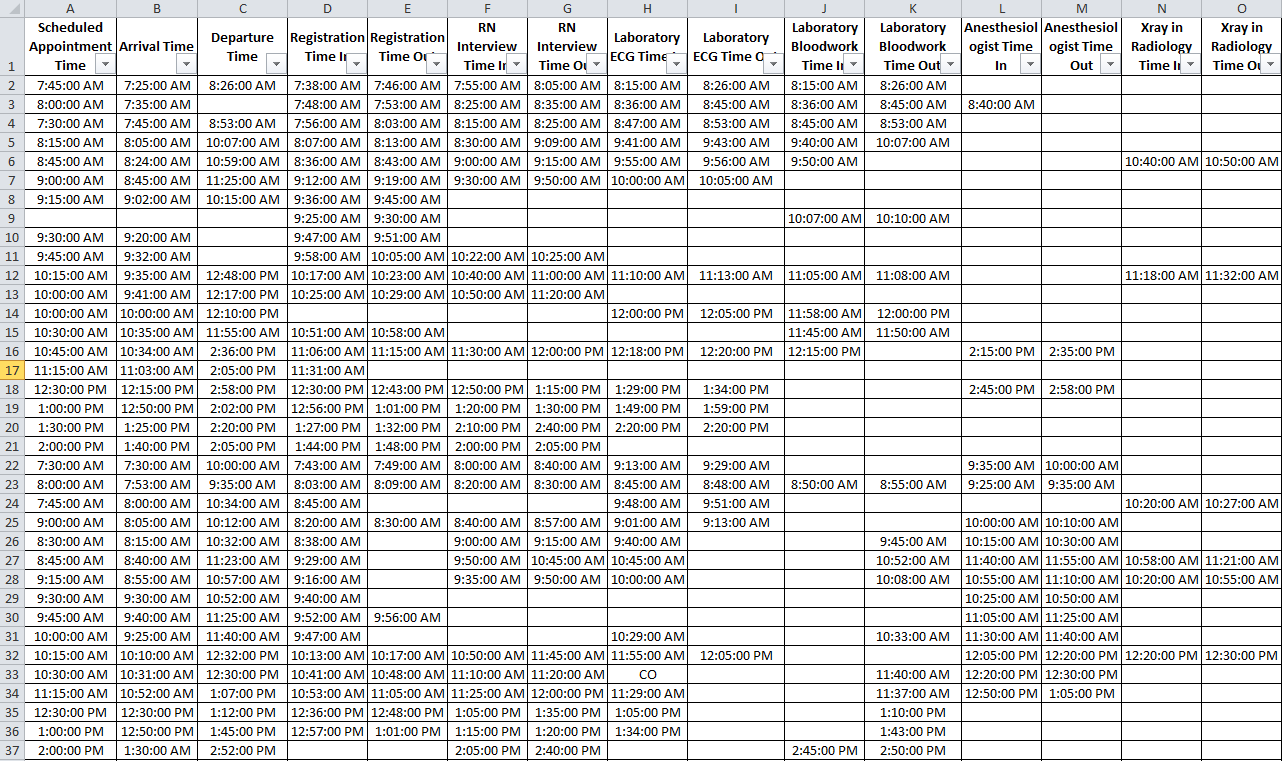
\includegraphics[scale=0.5]{dataanalysis.png}	

		\subsubsection{Outputs}
		\begin{verbatim}
		Arrivals Arrivals 1 1 
		normal -0.29174028268551283 2.3924217394163332
		
		Registration Registration 2 1 
		exponential 0.1291895185862281 1.8370753084966731
		
		RNInterview RNInterview 2 1
		 exponential 0.73117223313687152 0.42447599189639101
		
		LaboratoryECG LaboratoryECG 2 1 
		exponential 0.28118448637316579 0.4501155689862455
		
		LaboratoryBloodwork LaboratoryBloodwork 2 1 
		exponential 0.28010597302504836 0.17162556614020963
	
		Anesthesiologist Anesthesiologist 2 1 
		exponential 0.5706126687435098 0.35373810618811924
		
		XrayinRadiology XrayinRadiology 2 1 
		exponential 1.1311403508771929 0.68121776229524544
		
		Station Name: Registration  Station Prerequesites: ['Registration']  
		Maximum Capacity: 2  Minimum Capacity: 1  Variance Type: exponential  
		Mean: 0.1291895185862281  Variance: 1.837075308496673
		Station Name: RNInterview  Station Prerequesites: ['RNInterview']  
		Maximum Capacity: 2  Minimum Capacity: 1  Variance Type: exponential 
		 Mean: 0.7311722331368715  Variance: 0.424475991896391
		Station Name: LaboratoryECG  Station Prerequesites: ['LaboratoryECG'] 
		 Maximum Capacity: 2  Minimum Capacity: 1  Variance Type: exponential  
		 Mean: 0.2811844863731658  Variance: 0.4501155689862455
		Station Name: LaboratoryBloodwork  Station Prerequesites: ['LaboratoryBloodwork']  
		Maximum Capacity: 2  Minimum Capacity: 1  Variance Type: exponential 
		 Mean: 0.28010597302504836  Variance: 0.17162556614020963
		Station Name: Anesthesiologist  Station Prerequesites: ['Anesthesiologist'] 
		 Maximum Capacity: 2  Minimum Capacity: 1  Variance Type: exponential 
		  Mean: 0.5706126687435098  Variance: 0.35373810618811924
		Station Name: XrayinRadiology  Station Prerequesites: ['XrayinRadiology'] 
		 Maximum Capacity: 2  Minimum Capacity: 1  Variance Type: exponential  
		 Mean: 1.131140350877193  Variance: 0.6812177622952454
		\end{verbatim}
		
		\subsection{Simulation Engine Test}\label{simulationtests}
		\subsubsection{Inputs for test\# 23}
		\begin{verbatim}
		Patient1 Registration,RNInterview,LaboratoryECG,LaboratoryBloodwork,
		Anesthesiologist,XrayinRadiology
		Patient2 Registration,RNInterview,LaboratoryECG,LaboratoryBloodwork,
		Anesthesiologist,XrayinRadiology
		Patient3 Registration,RNInterview,LaboratoryECG,LaboratoryBloodwork,
		Anesthesiologist,XrayinRadiology
		Patient4 Registration,RNInterview,LaboratoryECG,LaboratoryBloodwork,
		Anesthesiologist
		Patient5 Registration,RNInterview,LaboratoryECG,LaboratoryBloodwork,
		Anesthesiologist,XrayinRadiology
		Patient6 Registration,RNInterview,LaboratoryECG,LaboratoryBloodwork
		Patient7 Registration,RNInterview,LaboratoryECG,LaboratoryBloodwork,
		Anesthesiologist,XrayinRadiology
		Patient8 Registration,RNInterview,LaboratoryECG,LaboratoryBloodwork,
		Anesthesiologist,XrayinRadiology
		Patient9 Registration,RNInterview,LaboratoryECG,LaboratoryBloodwork,
		Anesthesiologist,XrayinRadiology
		Patient10 Registration,RNInterview,LaboratoryECG,LaboratoryBloodwork
		Patient11 Registration,RNInterview,LaboratoryECG,LaboratoryBloodwork,
		Anesthesiologist,XrayinRadiology
		Patient12 Registration,RNInterview,LaboratoryECG,LaboratoryBloodwork,
		Anesthesiologist
		Patient13 Registration,RNInterview,LaboratoryECG,LaboratoryBloodwork,
		Anesthesiologist,XrayinRadiology
		Patient14 Registration,RNInterview,LaboratoryECG,LaboratoryBloodwork,
		Anesthesiologist,XrayinRadiology
		Patient15 Registration,RNInterview,LaboratoryECG,LaboratoryBloodwork,
		Anesthesiologist,XrayinRadiology
		Patient16 Registration,RNInterview,LaboratoryECG,LaboratoryBloodwork
		Patient17 Registration,RNInterview,LaboratoryECG,LaboratoryBloodwork
		Patient18 Registration,RNInterview,LaboratoryECG,LaboratoryBloodwork
		Patient19 Registration,RNInterview,LaboratoryECG,LaboratoryBloodwork,
		XrayinRadiology
		Patient20 Registration,RNInterview,LaboratoryECG,LaboratoryBloodwork
		Patient21 Registration,RNInterview,LaboratoryECG,LaboratoryBloodwork,
		XrayinRadiology
		Patient22 Registration,RNInterview,LaboratoryECG,LaboratoryBloodwork
		Patient23 Registration,RNInterview,LaboratoryECG,LaboratoryBloodwork,
		XrayinRadiology
		Patient24 Registration,RNInterview,LaboratoryECG,LaboratoryBloodwork
		Patient25 Registration,RNInterview,LaboratoryECG,LaboratoryBloodwork,
		XrayinRadiology
		
		NurseAshley 0,145,210,225 Registration
		NurseBrook 0,180,255,270 RNInterview
		NurseCameron 0,160,240,255 LaboratoryECG
		NurseDevon 0,140,225,240 LaboratoryBloodwork
		DoctorEli 0,165,0,15 Anesthesiologist
		TechFranky 0,180,360 XrayinRadiology
		NurseGeorge 0,180,180,180 Registration,RNInterview,
		LaboratoryECG,LaboratoryBloodwork
		\end{verbatim}
		
		\subsubsection{Outputs}
		\begin{verbatim}
		NurseAshley arriving at 8:00
		NurseBrook arriving at 8:00
		NurseCameron arriving at 8:00
		NurseDevon arriving at 8:00
		DoctorEli arriving at 8:00
		TechFranky arriving at 8:00
		NurseGeorge arriving at 8:00
		NurseAshley starting work at Registration 8:00
		NurseBrook starting work at RNInterview 8:00
		NurseCameron starting work at LaboratoryECG 8:00
		NurseDevon starting work at LaboratoryBloodwork 8:00
		DoctorEli starting work at Anesthesiologist 8:00
		TechFranky starting work at XrayinRadiology 8:00
		NurseGeorge starting work at Registration 8:00
		Patient1 arriving at 8:12
		Patient1 starting service at Registration 8:12
		Patient1 leaving service at Registration 8:20
		Patient1 starting service at RNInterview 8:24
		Patient1 leaving service at RNInterview 8:24
		Patient1 starting service at LaboratoryECG 8:26
		Patient1 leaving service at LaboratoryECG 8:29
		Patient2 arriving at 8:31
		Patient2 starting service at Registration 8:31
		Patient1 starting service at LaboratoryBloodwork 8:34
		Patient2 leaving service at Registration 8:40
		Patient3 arriving at 8:43
		Patient1 leaving service at LaboratoryBloodwork 8:43
		Patient3 starting service at Registration 8:43
		Patient1 starting service at Anesthesiologist 8:44
		Patient1 leaving service at Anesthesiologist 8:45
		Patient2 starting service at RNInterview 8:45
		Patient2 leaving service at RNInterview 8:45
		Patient1 starting service at XrayinRadiology 8:46
		Patient1 leaving service at XrayinRadiology 8:46
		Patient3 leaving service at Registration 8:47
		Patient2 starting service at LaboratoryECG 8:47
		Patient2 leaving service at LaboratoryECG 8:48
		Patient3 starting service at RNInterview 8:50
		Patient2 starting service at LaboratoryBloodwork 8:50
		Patient3 leaving service at RNInterview 8:50
		Patient3 starting service at LaboratoryECG 8:54
		Patient2 leaving service at LaboratoryBloodwork 8:57
		Patient3 leaving service at LaboratoryECG 8:57
		Patient4 arriving at 8:59
		Patient4 starting service at Registration 8:59
		Patient2 starting service at Anesthesiologist 8:59
		Patient2 leaving service at Anesthesiologist 9:00
		Patient3 starting service at LaboratoryBloodwork 9:01
		Patient3 leaving service at LaboratoryBloodwork 9:04
		Patient2 starting service at XrayinRadiology 9:05
		Patient2 leaving service at XrayinRadiology 9:05
		Patient3 starting service at Anesthesiologist 9:06
		Patient3 leaving service at Anesthesiologist 9:07
		Patient3 starting service at XrayinRadiology 9:12
		Patient5 arriving at 9:14
		Patient4 leaving service at Registration 9:14
		Patient3 leaving service at XrayinRadiology 9:14
		Patient5 starting service at Registration 9:14
		Patient4 starting service at RNInterview 9:18
		Patient4 leaving service at RNInterview 9:19
		Patient4 starting service at LaboratoryECG 9:22
		Patient5 leaving service at Registration 9:24
		Patient5 starting service at RNInterview 9:26
		Patient5 leaving service at RNInterview 9:26
		Patient6 arriving at 9:32
		Patient6 starting service at Registration 9:32
		Patient4 leaving service at LaboratoryECG 9:34
		Patient5 starting service at LaboratoryECG 9:34
		Patient5 leaving service at LaboratoryECG 9:34
		Patient6 leaving service at Registration 9:35
		Patient4 starting service at LaboratoryBloodwork 9:36
		Patient6 starting service at RNInterview 9:39
		Patient4 leaving service at LaboratoryBloodwork 9:40
		Patient5 starting service at LaboratoryBloodwork 9:40
		Patient5 leaving service at LaboratoryBloodwork 9:45
		Patient4 starting service at Anesthesiologist 9:45
		Patient4 leaving service at Anesthesiologist 9:46
		Patient7 arriving at 9:49
		Patient7 starting service at Registration 9:49
		Patient5 starting service at Anesthesiologist 9:49
		Patient5 leaving service at Anesthesiologist 9:50
		Patient6 leaving service at RNInterview 9:51
		Patient6 starting service at LaboratoryECG 9:52
		Patient6 leaving service at LaboratoryECG 9:53
		Patient5 starting service at XrayinRadiology 9:53
		Patient6 starting service at LaboratoryBloodwork 9:55
		Patient6 leaving service at LaboratoryBloodwork 9:55
		Patient5 leaving service at XrayinRadiology 9:56
		Patient8 arriving at 10:00
		Patient7 leaving service at Registration 10:06
		Patient8 starting service at Registration 10:06
		Patient8 leaving service at Registration 10:06
		Patient8 starting service at RNInterview 10:08
		Patient8 leaving service at RNInterview 10:08
		Patient7 starting service at RNInterview 10:11
		Patient8 starting service at LaboratoryECG 10:11
		Patient7 leaving service at RNInterview 10:13
		Patient9 arriving at 10:16
		Patient9 starting service at Registration 10:16
		Patient8 leaving service at LaboratoryECG 10:19
		Patient7 starting service at LaboratoryECG 10:19
		NurseDevon leaving work at LaboratoryBloodwork 10:20
		Patient7 leaving service at LaboratoryECG 10:22
		Patient8 starting service at Anesthesiologist 10:22
		Patient9 leaving service at Registration 10:24
		Patient8 leaving service at Anesthesiologist 10:24
		Patient7 starting service at Anesthesiologist 10:24
		Patient7 leaving service at Anesthesiologist 10:25
		NurseAshley leaving work at Registration 10:25
		Patient9 starting service at RNInterview 10:25
		Patient9 leaving service at RNInterview 10:26
		Patient10 arriving at 10:28
		Patient10 starting service at Registration 10:28
		Patient8 starting service at XrayinRadiology 10:28
		Patient8 leaving service at XrayinRadiology 10:28
		Patient7 starting service at XrayinRadiology 10:28
		Patient7 leaving service at XrayinRadiology 10:29
		Patient9 starting service at LaboratoryECG 10:31
		Patient10 leaving service at Registration 10:35
		Patient9 leaving service at LaboratoryECG 10:35
		NurseDevon starting work at LaboratoryBloodwork 10:35
		Patient8 starting service at LaboratoryBloodwork 10:36
		Patient8 leaving service at LaboratoryBloodwork 10:38
		Patient10 starting service at RNInterview 10:38
		Patient7 starting service at LaboratoryBloodwork 10:38
		Patient10 leaving service at RNInterview 10:40
		Patient7 leaving service at LaboratoryBloodwork 10:40
		NurseCameron leaving work at LaboratoryECG 10:40
		NurseAshley starting work at Registration 10:40
		Patient9 starting service at LaboratoryBloodwork 10:40
		Patient11 arriving at 10:43
		Patient11 starting service at Registration 10:43
		Patient11 leaving service at Registration 10:43
		Patient9 leaving service at LaboratoryBloodwork 10:45
		DoctorEli leaving work at Anesthesiologist 10:45
		Patient10 starting service at LaboratoryBloodwork 10:45
		Patient11 starting service at RNInterview 10:47
		Patient9 starting service at XrayinRadiology 10:47
		Patient9 leaving service at XrayinRadiology 10:47
		Patient11 leaving service at RNInterview 10:48
		Patient10 leaving service at LaboratoryBloodwork 10:51
		Patient11 starting service at LaboratoryBloodwork 10:53
		Patient11 leaving service at LaboratoryBloodwork 10:55
		NurseCameron starting work at LaboratoryECG 10:55
		Patient11 starting service at XrayinRadiology 10:56
		Patient11 leaving service at XrayinRadiology 10:56
		Patient10 starting service at LaboratoryECG 10:58
		NurseBrook leaving work at RNInterview 11:00
		TechFranky leaving work at XrayinRadiology 11:00
		NurseGeorge leaving work at Registration 11:00
		DoctorEli starting work at Anesthesiologist 11:00
		DoctorEli leaving work at Anesthesiologist 11:00
		Patient12 arriving at 11:01
		Patient12 starting service at Registration 11:01
		Patient12 leaving service at Registration 11:11
		Patient10 leaving service at LaboratoryECG 11:12
		Patient11 starting service at LaboratoryECG 11:12
		NurseBrook starting work at RNInterview 11:15
		TechFranky starting work at XrayinRadiology 11:15
		DoctorEli starting work at Anesthesiologist 11:15
		NurseGeorge starting work at RNInterview 11:15
		Patient9 starting service at Anesthesiologist 11:16
		Patient13 arriving at 11:17
		Patient13 starting service at Registration 11:17
		Patient9 leaving service at Anesthesiologist 11:18
		Patient13 leaving service at Registration 11:18
		Patient13 starting service at RNInterview 11:21
		Patient13 leaving service at RNInterview 11:23
		Patient11 leaving service at LaboratoryECG 11:24
		Patient12 starting service at LaboratoryECG 11:24
		Patient11 starting service at Anesthesiologist 11:27
		Patient12 leaving service at LaboratoryECG 11:29
		Patient11 leaving service at Anesthesiologist 11:29
		Patient13 starting service at LaboratoryECG 11:29
		DoctorEli leaving work at Anesthesiologist 11:30
		Patient14 arriving at 11:32
		Patient14 starting service at Registration 11:32
		Patient12 starting service at LaboratoryBloodwork 11:33
		Patient13 leaving service at LaboratoryECG 11:35
		Patient12 leaving service at LaboratoryBloodwork 11:36
		Patient13 starting service at LaboratoryBloodwork 11:36
		Patient13 leaving service at LaboratoryBloodwork 11:37
		Patient14 leaving service at Registration 11:38
		Patient13 starting service at XrayinRadiology 11:38
		Patient13 leaving service at XrayinRadiology 11:38
		Patient14 starting service at RNInterview 11:39
		Patient14 leaving service at RNInterview 11:39
		Patient14 starting service at LaboratoryECG 11:40
		Patient12 starting service at RNInterview 11:42
		Patient15 arriving at 11:44
		Patient12 leaving service at RNInterview 11:44
		Patient15 starting service at Registration 11:44
		DoctorEli starting work at Anesthesiologist 11:45
		Patient13 starting service at Anesthesiologist 11:46
		Patient13 leaving service at Anesthesiologist 11:46
		Patient14 leaving service at LaboratoryECG 11:49
		Patient15 leaving service at Registration 11:49
		Patient12 starting service at Anesthesiologist 11:49
		Patient12 leaving service at Anesthesiologist 11:49
		Patient14 starting service at LaboratoryBloodwork 11:52
		Patient15 starting service at RNInterview 11:52
		Patient15 leaving service at RNInterview 11:52
		Patient15 starting service at LaboratoryECG 11:55
		Patient16 arriving at 11:58
		Patient16 starting service at Registration 11:58
		Patient15 leaving service at LaboratoryECG 12:01
		Patient14 leaving service at LaboratoryBloodwork 12:03
		Patient16 leaving service at Registration 12:05
		Patient15 starting service at LaboratoryBloodwork 12:05
		Patient14 starting service at Anesthesiologist 12:05
		Patient15 leaving service at LaboratoryBloodwork 12:05
		Patient14 leaving service at Anesthesiologist 12:06
		Patient16 starting service at RNInterview 12:07
		Patient16 leaving service at RNInterview 12:08
		Patient15 starting service at Anesthesiologist 12:09
		Patient14 starting service at XrayinRadiology 12:09
		Patient15 leaving service at Anesthesiologist 12:10
		Patient16 starting service at LaboratoryECG 12:10
		Patient14 leaving service at XrayinRadiology 12:11
		Patient16 leaving service at LaboratoryECG 12:13
		Patient15 starting service at XrayinRadiology 12:13
		Patient15 leaving service at XrayinRadiology 12:13
		Patient16 starting service at LaboratoryBloodwork 12:15
		Patient16 leaving service at LaboratoryBloodwork 12:18
		Patient17 arriving at 12:20
		Patient17 starting service at Registration 12:20
		Patient17 leaving service at Registration 12:27
		Patient17 starting service at RNInterview 12:30
		Patient17 leaving service at RNInterview 12:31
		Patient18 arriving at 12:34
		Patient18 starting service at Registration 12:34
		Patient18 leaving service at Registration 12:34
		Patient17 starting service at LaboratoryECG 12:36
		Patient18 starting service at RNInterview 12:37
		Patient18 leaving service at RNInterview 12:38
		Patient17 leaving service at LaboratoryECG 12:39
		Patient18 starting service at LaboratoryECG 12:42
		Patient17 starting service at LaboratoryBloodwork 12:42
		Patient17 leaving service at LaboratoryBloodwork 12:44
		Patient19 arriving at 12:45
		Patient19 starting service at Registration 12:45
		Patient18 leaving service at LaboratoryECG 12:47
		Patient18 starting service at LaboratoryBloodwork 12:48
		Patient18 leaving service at LaboratoryBloodwork 12:48
		Patient20 arriving at 13:00
		Patient19 leaving service at Registration 13:03
		Patient20 starting service at Registration 13:03
		Patient20 leaving service at Registration 13:04
		Patient20 starting service at RNInterview 13:06
		Patient20 leaving service at RNInterview 13:06
		Patient19 starting service at RNInterview 13:07
		Patient19 leaving service at RNInterview 13:08
		Patient20 starting service at LaboratoryECG 13:09
		Patient21 arriving at 13:14
		Patient21 starting service at Registration 13:14
		Patient21 leaving service at Registration 13:16
		Patient21 starting service at RNInterview 13:17
		Patient20 leaving service at LaboratoryECG 13:18
		Patient21 leaving service at RNInterview 13:18
		Patient19 starting service at LaboratoryECG 13:18
		Patient20 starting service at LaboratoryBloodwork 13:23
		Patient22 arriving at 13:25
		Patient22 starting service at Registration 13:25
		Patient19 leaving service at LaboratoryECG 13:26
		Patient20 leaving service at LaboratoryBloodwork 13:26
		Patient21 starting service at LaboratoryECG 13:26
		Patient22 leaving service at Registration 13:28
		Patient21 leaving service at LaboratoryECG 13:28
		Patient19 starting service at LaboratoryBloodwork 13:28
		Patient22 starting service at RNInterview 13:29
		Patient22 leaving service at RNInterview 13:30
		Patient19 leaving service at LaboratoryBloodwork 13:31
		Patient22 starting service at LaboratoryECG 13:31
		Patient21 starting service at LaboratoryBloodwork 13:31
		Patient21 leaving service at LaboratoryBloodwork 13:31
		Patient21 starting service at XrayinRadiology 13:33
		Patient21 leaving service at XrayinRadiology 13:33
		Patient19 starting service at XrayinRadiology 13:36
		Patient19 leaving service at XrayinRadiology 13:37
		Patient22 leaving service at LaboratoryECG 13:40
		Patient22 starting service at LaboratoryBloodwork 13:41
		Patient23 arriving at 13:47
		Patient23 starting service at Registration 13:47
		Patient23 leaving service at Registration 13:49
		Patient22 leaving service at LaboratoryBloodwork 13:51
		Patient23 starting service at RNInterview 13:52
		Patient23 leaving service at RNInterview 13:53
		Patient23 starting service at LaboratoryECG 13:57
		Patient23 leaving service at LaboratoryECG 13:58
		Patient24 arriving at 14:00
		Patient24 starting service at Registration 14:00
		Patient23 starting service at LaboratoryBloodwork 14:01
		Patient23 leaving service at LaboratoryBloodwork 14:01
		Patient24 leaving service at Registration 14:03
		Patient23 starting service at XrayinRadiology 14:03
		Patient23 leaving service at XrayinRadiology 14:03
		Patient24 starting service at RNInterview 14:07
		Patient24 leaving service at RNInterview 14:09
		NurseAshley leaving work at Registration 14:10
		Patient24 starting service at LaboratoryECG 14:11
		Patient25 arriving at 14:13
		Patient25 starting service at RNInterview 14:13
		Patient25 leaving service at RNInterview 14:13
		NurseGeorge leaving work at RNInterview 14:15
		NurseDevon leaving work at LaboratoryBloodwork 14:20
		Patient24 leaving service at LaboratoryECG 14:21
		Patient25 starting service at LaboratoryECG 14:21
		Patient25 leaving service at LaboratoryECG 14:21
		NurseAshley starting work at Registration 14:25
		Patient25 starting service at XrayinRadiology 14:25
		Patient25 leaving service at XrayinRadiology 14:25
		NurseGeorge starting work at LaboratoryECG 14:30
		Patient25 starting service at Registration 14:33
		NurseDevon starting work at LaboratoryBloodwork 14:35
		Patient24 starting service at LaboratoryBloodwork 14:36
		Patient24 leaving service at LaboratoryBloodwork 14:36
		Patient25 leaving service at Registration 14:37
		Patient25 starting service at LaboratoryBloodwork 14:38
		Patient25 leaving service at LaboratoryBloodwork 14:44
		NurseCameron going home at 14:55
		NurseBrook going home at 15:30
		\end{verbatim}
		
		\subsubsection{Inputs for test\# 24}
		\begin{verbatim}
		Patient1 Registration,RNInterview,LaboratoryECG,LaboratoryBloodwork,
		Anesthesiologist,XrayinRadiology
		Patient2 Registration,RNInterview,LaboratoryECG,LaboratoryBloodwork,
		Anesthesiologist,XrayinRadiology
		Patient3 Registration,RNInterview,LaboratoryECG,LaboratoryBloodwork,
		Anesthesiologist,XrayinRadiology
		Patient4 Registration,RNInterview,LaboratoryECG,LaboratoryBloodwork,
		Anesthesiologist
		Patient5 Registration,RNInterview,LaboratoryECG,LaboratoryBloodwork,
		Anesthesiologist,XrayinRadiology
		Patient6 Registration,RNInterview,LaboratoryECG,LaboratoryBloodwork
		Patient7 Registration,RNInterview,LaboratoryECG,LaboratoryBloodwork,
		Anesthesiologist,XrayinRadiology
		Patient8 Registration,RNInterview,LaboratoryECG,LaboratoryBloodwork,
		Anesthesiologist,XrayinRadiology
		Patient9 Registration,RNInterview,LaboratoryECG,LaboratoryBloodwork,
		Anesthesiologist,XrayinRadiology
		Patient10 Registration,RNInterview,LaboratoryECG,LaboratoryBloodwork
		Patient11 Registration,RNInterview,LaboratoryECG,LaboratoryBloodwork,
		Anesthesiologist,XrayinRadiology
		Patient12 Registration,RNInterview,LaboratoryECG,LaboratoryBloodwork,
		Anesthesiologist
		Patient13 Registration,RNInterview,LaboratoryECG,LaboratoryBloodwork,
		Anesthesiologist,XrayinRadiology
		Patient14 Registration,RNInterview,LaboratoryECG,LaboratoryBloodwork,
		Anesthesiologist,XrayinRadiology
		Patient15 Registration,RNInterview,LaboratoryECG,LaboratoryBloodwork,
		Anesthesiologist,XrayinRadiology
		Patient16 Registration,RNInterview,LaboratoryECG,LaboratoryBloodwork
		Patient17 Registration,RNInterview,LaboratoryECG,LaboratoryBloodwork
		Patient18 Registration,RNInterview,LaboratoryECG,LaboratoryBloodwork
		Patient19 Registration,RNInterview,LaboratoryECG,LaboratoryBloodwork,
		XrayinRadiology
		Patient20 Registration,RNInterview,LaboratoryECG,LaboratoryBloodwork
		Patient21 Registration,RNInterview,LaboratoryECG,LaboratoryBloodwork,
		XrayinRadiology
		Patient22 Registration,RNInterview,LaboratoryECG,LaboratoryBloodwork
		Patient23 Registration,RNInterview,LaboratoryECG,LaboratoryBloodwork,
		XrayinRadiology
		Patient24 Registration,RNInterview,LaboratoryECG,LaboratoryBloodwork
		Patient25 Registration,RNInterview,LaboratoryECG,LaboratoryBloodwork,
		XrayinRadiology
		Patient26 Registration,RNInterview,LaboratoryECG,LaboratoryBloodwork,
		Anesthesiologist,XrayinRadiology
		Patient27 Registration,RNInterview,LaboratoryECG,LaboratoryBloodwork,
		Anesthesiologist,XrayinRadiology
		Patient28 Registration,RNInterview,LaboratoryECG,LaboratoryBloodwork,
		Anesthesiologist,XrayinRadiology
		Patient29 Registration,RNInterview,LaboratoryECG,LaboratoryBloodwork,
		Anesthesiologist
		Patient30 Registration,RNInterview,LaboratoryECG,LaboratoryBloodwork,
		Anesthesiologist,XrayinRadiology
		Patient31 Registration,RNInterview,LaboratoryECG,LaboratoryBloodwork
		Patient32 Registration,RNInterview,LaboratoryECG,LaboratoryBloodwork,
		Anesthesiologist,XrayinRadiology
		Patient33 Registration,RNInterview,LaboratoryECG,LaboratoryBloodwork,
		Anesthesiologist,XrayinRadiology
		Patient34 Registration,RNInterview,LaboratoryECG,LaboratoryBloodwork,
		Anesthesiologist,XrayinRadiology
		Patient35 Registration,RNInterview,LaboratoryECG,LaboratoryBloodwork
		Patient36 Registration,RNInterview,LaboratoryECG,LaboratoryBloodwork,
		Anesthesiologist,XrayinRadiology
		Patient37 Registration,RNInterview,LaboratoryECG,LaboratoryBloodwork,
		Anesthesiologist
		Patient38 Registration,RNInterview,LaboratoryECG,LaboratoryBloodwork,
		Anesthesiologist,XrayinRadiology
		Patient39 Registration,RNInterview,LaboratoryECG,LaboratoryBloodwork,
		Anesthesiologist,XrayinRadiology
		Patient40 Registration,RNInterview,LaboratoryECG,LaboratoryBloodwork,
		Anesthesiologist,XrayinRadiology
		Patient41 Registration,RNInterview,LaboratoryECG,LaboratoryBloodwork
		Patient42 Registration,RNInterview,LaboratoryECG,LaboratoryBloodwork
		Patient43 Registration,RNInterview,LaboratoryECG,LaboratoryBloodwork
		Patient44 Registration,RNInterview,LaboratoryECG,LaboratoryBloodwork,
		XrayinRadiology
		Patient45 Registration,RNInterview,LaboratoryECG,LaboratoryBloodwork
		Patient46 Registration,RNInterview,LaboratoryECG,LaboratoryBloodwork,
		XrayinRadiology
		Patient47 Registration,RNInterview,LaboratoryECG,LaboratoryBloodwork
		Patient48 Registration,RNInterview,LaboratoryECG,LaboratoryBloodwork,
		XrayinRadiology
		Patient49 Registration,RNInterview,LaboratoryECG,LaboratoryBloodwork
		Patient50 Registration,RNInterview,LaboratoryECG,LaboratoryBloodwork,
		XrayinRadiology
		
		NurseAshley 0,145,210,225 Registration
		NurseBrook 0,180,255,270 RNInterview
		NurseCameron 0,160,240,255 LaboratoryECG
		NurseDevon 0,140,225,240 LaboratoryBloodwork
		DoctorEli 0,165,0,15 Anesthesiologist
		TechFranky 0,180,360 XrayinRadiology
		NurseGeorge 0,180,180,180 Registration,
		RNInterview,LaboratoryECG,LaboratoryBloodwork
		\end{verbatim}
		\subsubsection{Outputs}
		\begin{verbatim}
		NurseAshley arriving at 8:00
		NurseBrook arriving at 8:00
		NurseCameron arriving at 8:00
		NurseDevon arriving at 8:00
		DoctorEli arriving at 8:00
		TechFranky arriving at 8:00
		NurseGeorge arriving at 8:00
		NurseAshley starting work at Registration 8:00
		NurseBrook starting work at RNInterview 8:00
		NurseCameron starting work at LaboratoryECG 8:00
		NurseDevon starting work at LaboratoryBloodwork 8:00
		DoctorEli starting work at Anesthesiologist 8:00
		TechFranky starting work at XrayinRadiology 8:00
		NurseGeorge starting work at Registration 8:00
		Patient1 arriving at 8:17
		Patient1 starting service at Registration 8:17
		Patient1 leaving service at Registration 8:20
		Patient1 starting service at RNInterview 8:23
		Patient1 leaving service at RNInterview 8:23
		Patient1 starting service at LaboratoryECG 8:27
		Patient1 leaving service at LaboratoryECG 8:27
		Patient2 arriving at 8:30
		Patient2 starting service at Registration 8:30
		Patient1 starting service at LaboratoryBloodwork 8:32
		Patient2 leaving service at Registration 8:36
		Patient1 leaving service at LaboratoryBloodwork 8:38
		Patient2 starting service at RNInterview 8:39
		Patient2 leaving service at RNInterview 8:40
		Patient1 starting service at Anesthesiologist 8:41
		Patient1 leaving service at Anesthesiologist 8:42
		Patient2 starting service at LaboratoryECG 8:43
		Patient3 arriving at 8:45
		Patient3 starting service at Registration 8:45
		Patient1 starting service at XrayinRadiology 8:47
		Patient1 leaving service at XrayinRadiology 8:48
		Patient2 leaving service at LaboratoryECG 8:55
		Patient3 leaving service at Registration 8:57
		Patient3 starting service at RNInterview 8:58
		Patient3 leaving service at RNInterview 8:58
		Patient2 starting service at LaboratoryBloodwork 8:59
		Patient4 arriving at 9:01
		Patient4 starting service at Registration 9:01
		Patient3 starting service at LaboratoryECG 9:03
		Patient4 leaving service at Registration 9:04
		Patient2 leaving service at LaboratoryBloodwork 9:07
		Patient4 starting service at RNInterview 9:07
		Patient3 leaving service at LaboratoryECG 9:09
		Patient4 leaving service at RNInterview 9:10
		Patient2 starting service at Anesthesiologist 9:10
		Patient2 leaving service at Anesthesiologist 9:11
		Patient3 starting service at LaboratoryBloodwork 9:12
		Patient2 starting service at XrayinRadiology 9:13
		Patient5 arriving at 9:14
		Patient5 starting service at Registration 9:14
		Patient4 starting service at LaboratoryECG 9:15
		Patient2 leaving service at XrayinRadiology 9:16
		Patient4 leaving service at LaboratoryECG 9:17
		Patient5 leaving service at Registration 9:18
		Patient3 leaving service at LaboratoryBloodwork 9:19
		Patient4 starting service at LaboratoryBloodwork 9:19
		Patient5 starting service at RNInterview 9:20
		Patient3 starting service at Anesthesiologist 9:20
		Patient5 leaving service at RNInterview 9:20
		Patient3 leaving service at Anesthesiologist 9:20
		Patient3 starting service at XrayinRadiology 9:23
		Patient3 leaving service at XrayinRadiology 9:23
		Patient4 leaving service at LaboratoryBloodwork 9:24
		Patient6 arriving at 9:25
		Patient6 starting service at Registration 9:25
		Patient5 starting service at LaboratoryECG 9:25
		Patient6 leaving service at Registration 9:26
		Patient6 starting service at RNInterview 9:27
		Patient6 leaving service at RNInterview 9:27
		Patient4 starting service at Anesthesiologist 9:28
		Patient4 leaving service at Anesthesiologist 9:29
		Patient5 leaving service at LaboratoryECG 9:44
		Patient6 starting service at LaboratoryECG 9:44
		Patient7 arriving at 9:45
		Patient6 leaving service at LaboratoryECG 9:45
		Patient7 starting service at Registration 9:45
		Patient5 starting service at LaboratoryBloodwork 9:45
		Patient7 leaving service at Registration 9:48
		Patient7 starting service at RNInterview 9:51
		Patient7 leaving service at RNInterview 9:53
		Patient5 leaving service at LaboratoryBloodwork 9:55
		Patient6 starting service at LaboratoryBloodwork 9:55
		Patient7 starting service at LaboratoryECG 9:57
		Patient5 starting service at Anesthesiologist 9:58
		Patient5 leaving service at Anesthesiologist 9:59
		Patient8 arriving at 10:03
		Patient6 leaving service at LaboratoryBloodwork 10:03
		Patient8 starting service at Registration 10:03
		Patient5 starting service at XrayinRadiology 10:03
		Patient5 leaving service at XrayinRadiology 10:04
		Patient7 leaving service at LaboratoryECG 10:05
		Patient7 starting service at LaboratoryBloodwork 10:07
		Patient8 leaving service at Registration 10:13
		Patient9 arriving at 10:14
		Patient9 starting service at Registration 10:14
		Patient7 leaving service at LaboratoryBloodwork 10:15
		Patient8 starting service at RNInterview 10:16
		Patient7 starting service at Anesthesiologist 10:16
		Patient8 leaving service at RNInterview 10:16
		Patient7 leaving service at Anesthesiologist 10:16
		Patient7 starting service at XrayinRadiology 10:19
		Patient7 leaving service at XrayinRadiology 10:20
		NurseDevon leaving work at LaboratoryBloodwork 10:20
		Patient8 starting service at LaboratoryECG 10:20
		Patient8 leaving service at LaboratoryECG 10:22
		Patient8 starting service at Anesthesiologist 10:23
		Patient9 leaving service at Registration 10:25
		Patient8 leaving service at Anesthesiologist 10:25
		NurseAshley leaving work at Registration 10:25
		Patient9 starting service at RNInterview 10:27
		Patient8 starting service at XrayinRadiology 10:27
		Patient9 leaving service at RNInterview 10:28
		Patient10 arriving at 10:29
		Patient10 starting service at Registration 10:29
		Patient8 leaving service at XrayinRadiology 10:30
		Patient10 leaving service at Registration 10:30
		Patient10 starting service at RNInterview 10:31
		Patient10 leaving service at RNInterview 10:31
		Patient9 starting service at LaboratoryECG 10:32
		Patient9 leaving service at LaboratoryECG 10:34
		Patient10 starting service at LaboratoryECG 10:34
		NurseDevon starting work at LaboratoryBloodwork 10:35
		Patient8 starting service at LaboratoryBloodwork 10:37
		NurseAshley starting work at Registration 10:40
		Patient11 arriving at 10:44
		Patient11 starting service at Registration 10:44
		Patient10 leaving service at LaboratoryECG 10:45
		DoctorEli leaving work at Anesthesiologist 10:45
		NurseCameron leaving work at LaboratoryECG 10:45
		Patient11 leaving service at Registration 10:48
		Patient8 leaving service at LaboratoryBloodwork 10:50
		Patient9 starting service at LaboratoryBloodwork 10:50
		Patient9 leaving service at LaboratoryBloodwork 10:51
		Patient11 starting service at RNInterview 10:51
		Patient10 starting service at LaboratoryBloodwork 10:51
		Patient11 leaving service at RNInterview 10:52
		Patient10 leaving service at LaboratoryBloodwork 10:53
		Patient9 starting service at XrayinRadiology 10:54
		Patient11 starting service at LaboratoryBloodwork 10:54
		Patient9 leaving service at XrayinRadiology 10:55
		Patient12 arriving at 10:59
		Patient12 starting service at Registration 10:59
		NurseBrook leaving work at RNInterview 11:00
		TechFranky leaving work at XrayinRadiology 11:00
		DoctorEli starting work at Anesthesiologist 11:00
		NurseCameron starting work at LaboratoryECG 11:00
		DoctorEli leaving work at Anesthesiologist 11:00
		Patient11 leaving service at LaboratoryBloodwork 11:02
		Patient12 leaving service at Registration 11:03
		NurseGeorge leaving work at Registration 11:03
		Patient12 starting service at LaboratoryECG 11:05
		Patient12 leaving service at LaboratoryECG 11:09
		Patient11 starting service at LaboratoryECG 11:09
		Patient11 leaving service at LaboratoryECG 11:10
		Patient13 arriving at 11:13
		Patient13 starting service at Registration 11:13
		Patient12 starting service at LaboratoryBloodwork 11:13
		Patient13 leaving service at Registration 11:13
		Patient13 starting service at LaboratoryECG 11:14
		Patient12 leaving service at LaboratoryBloodwork 11:15
		NurseBrook starting work at RNInterview 11:15
		TechFranky starting work at XrayinRadiology 11:15
		DoctorEli starting work at Anesthesiologist 11:15
		Patient9 starting service at Anesthesiologist 11:17
		NurseGeorge starting work at RNInterview 11:18
		Patient9 leaving service at Anesthesiologist 11:19
		Patient11 starting service at Anesthesiologist 11:19
		Patient11 leaving service at Anesthesiologist 11:20
		Patient12 starting service at Anesthesiologist 11:20
		Patient13 leaving service at LaboratoryECG 11:22
		Patient12 leaving service at Anesthesiologist 11:22
		Patient11 starting service at XrayinRadiology 11:22
		Patient11 leaving service at XrayinRadiology 11:22
		Patient13 starting service at LaboratoryBloodwork 11:25
		Patient12 starting service at RNInterview 11:27
		Patient12 leaving service at RNInterview 11:27
		Patient14 arriving at 11:29
		Patient13 leaving service at LaboratoryBloodwork 11:29
		Patient14 starting service at Registration 11:29
		DoctorEli leaving work at Anesthesiologist 11:30
		Patient13 starting service at XrayinRadiology 11:34
		Patient14 leaving service at Registration 11:36
		Patient13 leaving service at XrayinRadiology 11:36
		Patient14 starting service at RNInterview 11:40
		Patient14 leaving service at RNInterview 11:43
		Patient13 starting service at RNInterview 11:43
		Patient13 leaving service at RNInterview 11:43
		DoctorEli starting work at Anesthesiologist 11:45
		Patient15 arriving at 11:47
		Patient15 starting service at Registration 11:47
		Patient14 starting service at LaboratoryECG 11:47
		Patient14 leaving service at LaboratoryECG 11:47
		Patient13 starting service at Anesthesiologist 11:48
		Patient14 starting service at LaboratoryBloodwork 11:50
		Patient13 leaving service at Anesthesiologist 11:53
		Patient16 arriving at 11:56
		Patient14 leaving service at LaboratoryBloodwork 11:57
		Patient14 starting service at Anesthesiologist 12:01
		Patient15 leaving service at Registration 12:02
		Patient14 leaving service at Anesthesiologist 12:02
		Patient16 starting service at Registration 12:02
		Patient15 starting service at RNInterview 12:03
		Patient15 leaving service at RNInterview 12:05
		Patient14 starting service at XrayinRadiology 12:06
		Patient14 leaving service at XrayinRadiology 12:06
		Patient16 leaving service at Registration 12:07
		Patient15 starting service at LaboratoryECG 12:10
		Patient16 starting service at RNInterview 12:10
		Patient16 leaving service at RNInterview 12:13
		Patient17 arriving at 12:14
		Patient17 starting service at Registration 12:14
		Patient17 leaving service at Registration 12:15
		Patient17 starting service at RNInterview 12:17
		Patient17 leaving service at RNInterview 12:20
		Patient15 leaving service at LaboratoryECG 12:22
		Patient16 starting service at LaboratoryECG 12:22
		Patient15 starting service at LaboratoryBloodwork 12:23
		Patient15 leaving service at LaboratoryBloodwork 12:25
		Patient18 arriving at 12:27
		Patient16 leaving service at LaboratoryECG 12:27
		Patient18 starting service at Registration 12:27
		Patient17 starting service at LaboratoryECG 12:27
		Patient15 starting service at Anesthesiologist 12:29
		Patient16 starting service at LaboratoryBloodwork 12:29
		Patient15 leaving service at Anesthesiologist 12:30
		Patient16 leaving service at LaboratoryBloodwork 12:31
		Patient15 starting service at XrayinRadiology 12:35
		Patient15 leaving service at XrayinRadiology 12:35
		Patient19 arriving at 12:47
		Patient17 leaving service at LaboratoryECG 12:47
		Patient17 starting service at LaboratoryBloodwork 12:48
		Patient17 leaving service at LaboratoryBloodwork 12:50
		Patient18 leaving service at Registration 12:52
		Patient19 starting service at Registration 12:52
		Patient19 leaving service at Registration 12:53
		Patient18 starting service at RNInterview 12:55
		Patient18 leaving service at RNInterview 12:56
		Patient19 starting service at RNInterview 12:56
		Patient19 leaving service at RNInterview 12:56
		Patient20 arriving at 12:58
		Patient20 starting service at Registration 12:58
		Patient18 starting service at LaboratoryECG 12:59
		Patient18 leaving service at LaboratoryECG 13:01
		Patient19 starting service at LaboratoryECG 13:01
		Patient20 leaving service at Registration 13:02
		Patient19 leaving service at LaboratoryECG 13:03
		Patient18 starting service at LaboratoryBloodwork 13:03
		Patient20 starting service at RNInterview 13:04
		Patient20 leaving service at RNInterview 13:04
		Patient18 leaving service at LaboratoryBloodwork 13:07
		Patient19 starting service at LaboratoryBloodwork 13:07
		Patient20 starting service at LaboratoryECG 13:08
		Patient19 leaving service at LaboratoryBloodwork 13:11
		Patient19 starting service at XrayinRadiology 13:12
		Patient19 leaving service at XrayinRadiology 13:12
		Patient20 leaving service at LaboratoryECG 13:13
		Patient20 starting service at LaboratoryBloodwork 13:18
		Patient21 arriving at 13:20
		Patient21 starting service at Registration 13:20
		Patient20 leaving service at LaboratoryBloodwork 13:21
		Patient22 arriving at 13:28
		Patient21 leaving service at Registration 13:37
		Patient22 starting service at Registration 13:37
		Patient21 starting service at RNInterview 13:39
		Patient21 leaving service at RNInterview 13:40
		Patient21 starting service at LaboratoryECG 13:45
		Patient23 arriving at 13:46
		Patient21 leaving service at LaboratoryECG 13:46
		Patient21 starting service at LaboratoryBloodwork 13:47
		Patient21 leaving service at LaboratoryBloodwork 13:50
		Patient21 starting service at XrayinRadiology 13:51
		Patient21 leaving service at XrayinRadiology 13:51
		Patient24 arriving at 14:00
		Patient22 leaving service at Registration 14:06
		Patient23 starting service at Registration 14:06
		Patient22 starting service at RNInterview 14:08
		Patient22 leaving service at RNInterview 14:08
		Patient22 starting service at LaboratoryECG 14:12
		Patient22 leaving service at LaboratoryECG 14:13
		Patient22 starting service at LaboratoryBloodwork 14:14
		Patient25 arriving at 14:16
		Patient23 leaving service at Registration 14:18
		NurseGeorge leaving work at RNInterview 14:18
		NurseAshley leaving work at Registration 14:18
		Patient24 starting service at Registration 14:18
		Patient23 starting service at RNInterview 14:20
		Patient23 leaving service at RNInterview 14:20
		Patient23 starting service at LaboratoryECG 14:24
		Patient23 leaving service at LaboratoryECG 14:25
		Patient24 leaving service at Registration 14:27
		Patient25 starting service at Registration 14:27
		Patient22 leaving service at LaboratoryBloodwork 14:28
		NurseDevon leaving work at LaboratoryBloodwork 14:28
		Patient23 starting service at XrayinRadiology 14:29
		Patient23 leaving service at XrayinRadiology 14:31
		Patient26 arriving at 14:32
		Patient26 starting service at RNInterview 14:32
		NurseGeorge starting work at LaboratoryECG 14:33
		Patient26 leaving service at RNInterview 14:35
		Patient24 starting service at RNInterview 14:35
		Patient24 leaving service at RNInterview 14:35
		Patient24 starting service at LaboratoryECG 14:38
		Patient27 arriving at 14:41
		Patient25 leaving service at Registration 14:41
		Patient27 starting service at RNInterview 14:41
		NurseAshley starting work at Registration 14:41
		Patient27 leaving service at RNInterview 14:43
		NurseDevon starting work at LaboratoryBloodwork 14:43
		Patient25 starting service at RNInterview 14:43
		Patient25 leaving service at RNInterview 14:43
		Patient23 starting service at LaboratoryBloodwork 14:44
		Patient23 leaving service at LaboratoryBloodwork 14:44
		Patient24 leaving service at LaboratoryECG 14:48
		Patient26 starting service at LaboratoryECG 14:48
		Patient24 starting service at LaboratoryBloodwork 14:53
		Patient24 leaving service at LaboratoryBloodwork 14:57
		Patient28 arriving at 14:59
		Patient28 starting service at Registration 14:59
		Patient26 leaving service at LaboratoryECG 15:01
		NurseCameron leaving work at LaboratoryECG 15:01
		Patient25 starting service at LaboratoryECG 15:01
		Patient26 starting service at LaboratoryBloodwork 15:02
		Patient25 leaving service at LaboratoryECG 15:03
		Patient26 leaving service at LaboratoryBloodwork 15:03
		Patient27 starting service at LaboratoryECG 15:03
		Patient25 starting service at LaboratoryBloodwork 15:04
		Patient26 starting service at Anesthesiologist 15:07
		Patient25 leaving service at LaboratoryBloodwork 15:09
		Patient26 leaving service at Anesthesiologist 15:10
		Patient27 leaving service at LaboratoryECG 15:11
		Patient28 leaving service at Registration 15:12
		Patient25 starting service at XrayinRadiology 15:12
		Patient27 starting service at LaboratoryBloodwork 15:12
		Patient25 leaving service at XrayinRadiology 15:12
		Patient27 leaving service at LaboratoryBloodwork 15:13
		Patient26 starting service at XrayinRadiology 15:13
		Patient26 leaving service at XrayinRadiology 15:13
		Patient27 starting service at Anesthesiologist 15:14
		Patient29 arriving at 15:15
		Patient29 starting service at Registration 15:15
		NurseCameron starting work at LaboratoryECG 15:16
		Patient28 starting service at RNInterview 15:16
		Patient29 leaving service at Registration 15:17
		Patient26 starting service at Registration 15:17
		Patient27 leaving service at Anesthesiologist 15:19
		Patient28 leaving service at RNInterview 15:21
		Patient29 starting service at RNInterview 15:21
		Patient29 leaving service at RNInterview 15:22
		Patient27 starting service at XrayinRadiology 15:24
		Patient27 leaving service at XrayinRadiology 15:24
		Patient28 starting service at LaboratoryECG 15:25
		Patient26 leaving service at Registration 15:26
		Patient28 leaving service at LaboratoryECG 15:29
		Patient27 starting service at Registration 15:29
		Patient29 starting service at LaboratoryECG 15:29
		NurseBrook leaving work at RNInterview 15:30
		Patient27 leaving service at Registration 15:31
		Patient28 starting service at LaboratoryBloodwork 15:31
		Patient29 leaving service at LaboratoryECG 15:32
		Patient30 arriving at 15:33
		Patient30 starting service at Registration 15:33
		Patient28 leaving service at LaboratoryBloodwork 15:34
		Patient28 starting service at Anesthesiologist 15:35
		Patient28 leaving service at Anesthesiologist 15:37
		Patient29 starting service at LaboratoryBloodwork 15:37
		Patient28 starting service at XrayinRadiology 15:39
		Patient28 leaving service at XrayinRadiology 15:39
		Patient31 arriving at 15:43
		Patient29 leaving service at LaboratoryBloodwork 15:43
		NurseBrook starting work at RNInterview 15:45
		Patient29 starting service at Anesthesiologist 15:48
		Patient29 leaving service at Anesthesiologist 15:50
		Patient30 leaving service at Registration 16:00
		Patient31 starting service at Registration 16:00
		Patient32 arriving at 16:01
		Patient30 starting service at RNInterview 16:03
		Patient31 leaving service at Registration 16:05
		Patient32 starting service at Registration 16:05
		Patient30 leaving service at RNInterview 16:06
		Patient31 starting service at RNInterview 16:08
		Patient31 leaving service at RNInterview 16:09
		Patient32 leaving service at Registration 16:10
		Patient30 starting service at LaboratoryECG 16:11
		Patient30 leaving service at LaboratoryECG 16:11
		Patient31 starting service at LaboratoryECG 16:11
		Patient33 arriving at 16:12
		Patient33 starting service at Registration 16:12
		Patient31 leaving service at LaboratoryECG 16:15
		Patient32 starting service at RNInterview 16:15
		Patient32 leaving service at RNInterview 16:15
		Patient30 starting service at LaboratoryBloodwork 16:16
		Patient32 starting service at LaboratoryECG 16:20
		Patient33 leaving service at Registration 16:21
		Patient33 starting service at RNInterview 16:23
		Patient33 leaving service at RNInterview 16:23
		Patient30 leaving service at LaboratoryBloodwork 16:28
		Patient31 starting service at LaboratoryBloodwork 16:28
		Patient31 leaving service at LaboratoryBloodwork 16:28
		Patient34 arriving at 16:29
		Patient34 starting service at Registration 16:29
		Patient30 starting service at Anesthesiologist 16:30
		Patient32 leaving service at LaboratoryECG 16:32
		Patient30 leaving service at Anesthesiologist 16:32
		Patient33 starting service at LaboratoryECG 16:32
		Patient33 leaving service at LaboratoryECG 16:32
		Patient33 starting service at LaboratoryBloodwork 16:33
		Patient30 starting service at XrayinRadiology 16:34
		Patient34 leaving service at Registration 16:35
		Patient33 leaving service at LaboratoryBloodwork 16:36
		Patient34 starting service at RNInterview 16:36
		Patient30 leaving service at XrayinRadiology 16:37
		Patient34 leaving service at RNInterview 16:37
		Patient32 starting service at LaboratoryBloodwork 16:37
		Patient33 starting service at Anesthesiologist 16:37
		Patient34 starting service at LaboratoryECG 16:38
		Patient33 leaving service at Anesthesiologist 16:39
		Patient34 leaving service at LaboratoryECG 16:42
		Patient32 leaving service at LaboratoryBloodwork 16:43
		Patient33 starting service at XrayinRadiology 16:43
		Patient33 leaving service at XrayinRadiology 16:43
		Patient34 starting service at LaboratoryBloodwork 16:44
		Patient35 arriving at 16:47
		Patient35 starting service at Registration 16:47
		Patient32 starting service at Anesthesiologist 16:48
		Patient32 leaving service at Anesthesiologist 16:48
		Patient34 leaving service at LaboratoryBloodwork 16:49
		Patient32 starting service at XrayinRadiology 16:50
		Patient32 leaving service at XrayinRadiology 16:52
		Patient34 starting service at Anesthesiologist 16:54
		Patient35 leaving service at Registration 16:55
		Patient34 leaving service at Anesthesiologist 16:56
		Patient35 starting service at RNInterview 16:57
		Patient35 leaving service at RNInterview 16:58
		Patient34 starting service at XrayinRadiology 16:58
		Patient34 leaving service at XrayinRadiology 16:59
		Patient36 arriving at 17:00
		Patient36 starting service at Registration 17:00
		Patient35 starting service at LaboratoryECG 17:00
		\end{verbatim}
		
		\subsubsection{Inputs for test\# 25}
		\begin{verbatim}
		Patient1 Registration,RNInterview,LaboratoryECG,LaboratoryBloodwork
		Patient2 Registration,RNInterview,LaboratoryECG,LaboratoryBloodwork
		Patient3 Registration,RNInterview,LaboratoryECG,LaboratoryBloodwork,
		Anesthesiologist,XrayinRadiology
		Patient4 Registration,RNInterview,LaboratoryECG,LaboratoryBloodwork,
		Anesthesiologist
		Patient5 Registration,RNInterview,LaboratoryECG,LaboratoryBloodwork,
		XrayinRadiology
		Patient6 Registration,RNInterview,LaboratoryECG,LaboratoryBloodwork
		Patient7 Registration,RNInterview,LaboratoryECG,LaboratoryBloodwork,
		Anesthesiologist,XrayinRadiology
		Patient8 Registration,RNInterview,LaboratoryECG,LaboratoryBloodwork,
		Anesthesiologist,XrayinRadiology
		Patient9 Registration,RNInterview,LaboratoryECG,LaboratoryBloodwork,
		Anesthesiologist,XrayinRadiology
		Patient10 Registration,RNInterview,LaboratoryECG,LaboratoryBloodwork
		Patient11 Registration,RNInterview,LaboratoryECG,LaboratoryBloodwork,
		Anesthesiologist,XrayinRadiology
		Patient12 Registration,RNInterview,LaboratoryECG,LaboratoryBloodwork,
		Anesthesiologist
		Patient13 Registration,RNInterview,LaboratoryECG,LaboratoryBloodwork,
		Anesthesiologist
		Patient14 Registration,RNInterview,LaboratoryECG,LaboratoryBloodwork,
		Anesthesiologist,XrayinRadiology
		Patient15 Registration,RNInterview,LaboratoryECG,LaboratoryBloodwork,
		Anesthesiologist
		Patient16 Registration,RNInterview,LaboratoryECG,LaboratoryBloodwork
		Patient17 Registration,RNInterview,LaboratoryECG,LaboratoryBloodwork
		Patient18 Registration,RNInterview,LaboratoryECG,LaboratoryBloodwork
		Patient19 Registration,RNInterview,LaboratoryECG,LaboratoryBloodwork,
		XrayinRadiology
		
		NurseAshley 0,80,120,220 Registration,RNInterview,LaboratoryECG,LaboratoryBloodwork,
		Anesthesiologist,XrayinRadiology
		NurseBrook 0,90,110,220 Registration,RNInterview,LaboratoryECG,LaboratoryBloodwork,
		Anesthesiologist,XrayinRadiology
		\end{verbatim}
		
		\subsubsection{Outputs}
		\begin{verbatim}
		NurseAshley arriving at 8:00
		NurseBrook arriving at 8:00
		NurseAshley starting work at Registration 8:00
		NurseBrook starting work at Registration 8:00
		Patient1 arriving at 8:21
		Patient1 starting service at Registration 8:21
		Patient1 leaving service at Registration 8:29
		Patient2 arriving at 8:31
		Patient2 starting service at Registration 8:31
		Patient2 leaving service at Registration 8:33
		Patient3 arriving at 8:43
		Patient3 starting service at Registration 8:43
		Patient3 leaving service at Registration 8:44
		Patient4 arriving at 8:59
		Patient4 starting service at Registration 8:59
		Patient4 leaving service at Registration 9:10
		Patient5 arriving at 9:12
		Patient5 starting service at Registration 9:12
		Patient5 leaving service at Registration 9:15
		NurseAshley leaving work at Registration 9:20
		Patient6 arriving at 9:30
		Patient6 starting service at Registration 9:30
		NurseAshley starting work at RNInterview 9:35
		Patient1 starting service at RNInterview 9:36
		Patient1 leaving service at RNInterview 9:37
		Patient2 starting service at RNInterview 9:37
		Patient2 leaving service at RNInterview 9:37
		Patient3 starting service at RNInterview 9:37
		Patient3 leaving service at RNInterview 9:37
		Patient5 starting service at RNInterview 9:37
		Patient5 leaving service at RNInterview 9:39
		Patient4 starting service at RNInterview 9:39
		Patient4 leaving service at RNInterview 9:40
		Patient7 arriving at 9:44
		Patient6 leaving service at Registration 9:48
		NurseBrook leaving work at Registration 9:48
		Patient7 starting service at Registration 9:48
		Patient6 starting service at RNInterview 9:52
		Patient6 leaving service at RNInterview 9:52
		Patient8 arriving at 9:54
		Patient7 leaving service at Registration 9:54
		Patient8 starting service at RNInterview 9:54
		Patient8 leaving service at RNInterview 9:54
		Patient7 starting service at RNInterview 9:56
		Patient7 leaving service at RNInterview 9:58
		NurseBrook starting work at RNInterview 10:03
		Patient9 arriving at 10:13
		Patient9 starting service at RNInterview 10:13
		Patient9 leaving service at RNInterview 10:15
		Patient10 arriving at 10:28
		Patient10 starting service at RNInterview 10:28
		Patient10 leaving service at RNInterview 10:29
		Patient11 arriving at 10:44
		Patient11 starting service at RNInterview 10:44
		Patient11 leaving service at RNInterview 10:45
		Patient12 arriving at 10:59
		Patient12 starting service at RNInterview 10:59
		Patient12 leaving service at RNInterview 10:59
		Patient13 arriving at 11:16
		Patient13 starting service at RNInterview 11:16
		Patient13 leaving service at RNInterview 11:16
		Patient14 arriving at 11:28
		Patient14 starting service at RNInterview 11:28
		Patient14 leaving service at RNInterview 11:29
		NurseAshley leaving work at RNInterview 11:35
		Patient15 arriving at 11:44
		Patient15 starting service at RNInterview 11:44
		Patient15 leaving service at RNInterview 11:45
		NurseAshley starting work at LaboratoryECG 11:50
		Patient3 starting service at LaboratoryECG 11:51
		NurseBrook leaving work at RNInterview 11:53
		Patient3 leaving service at LaboratoryECG 11:54
		Patient15 starting service at LaboratoryECG 11:54
		Patient15 leaving service at LaboratoryECG 11:55
		Patient13 starting service at LaboratoryECG 11:55
		Patient16 arriving at 11:58
		Patient13 leaving service at LaboratoryECG 12:04
		Patient8 starting service at LaboratoryECG 12:04
		Patient8 leaving service at LaboratoryECG 12:08
		NurseBrook starting work at LaboratoryECG 12:08
		Patient9 starting service at LaboratoryECG 12:08
		Patient9 leaving service at LaboratoryECG 12:08
		Patient10 starting service at LaboratoryECG 12:08
		Patient10 leaving service at LaboratoryECG 12:11
		Patient6 starting service at LaboratoryECG 12:11
		Patient17 arriving at 12:12
		Patient6 leaving service at LaboratoryECG 12:17
		Patient14 starting service at LaboratoryECG 12:17
		Patient14 leaving service at LaboratoryECG 12:27
		Patient11 starting service at LaboratoryECG 12:27
		Patient18 arriving at 12:28
		Patient11 leaving service at LaboratoryECG 12:28
		Patient1 starting service at LaboratoryECG 12:28
		Patient1 leaving service at LaboratoryECG 12:33
		Patient12 starting service at LaboratoryECG 12:33
		Patient12 leaving service at LaboratoryECG 12:36
		Patient4 starting service at LaboratoryECG 12:36
		Patient4 leaving service at LaboratoryECG 12:39
		Patient5 starting service at LaboratoryECG 12:39
		Patient19 arriving at 12:44
		Patient5 leaving service at LaboratoryECG 12:44
		Patient2 starting service at LaboratoryECG 12:44
		Patient2 leaving service at LaboratoryECG 12:50
		Patient7 starting service at LaboratoryECG 12:50
		Patient7 leaving service at LaboratoryECG 12:51
		Patient16 starting service at LaboratoryECG 12:51
		Patient16 leaving service at LaboratoryECG 13:00
		Patient17 starting service at LaboratoryECG 13:00
		Patient17 leaving service at LaboratoryECG 13:01
		Patient18 starting service at LaboratoryECG 13:01
		Patient18 leaving service at LaboratoryECG 13:03
		Patient19 starting service at LaboratoryECG 13:03
		Patient19 leaving service at LaboratoryECG 13:04
		NurseAshley leaving work at LaboratoryECG 15:30
		NurseAshley starting work at LaboratoryBloodwork 15:45
		Patient14 starting service at LaboratoryBloodwork 15:46
		NurseBrook leaving work at LaboratoryECG 15:48
		Patient14 leaving service at LaboratoryBloodwork 15:52
		Patient9 starting service at LaboratoryBloodwork 15:52
		Patient9 leaving service at LaboratoryBloodwork 15:52
		Patient19 starting service at LaboratoryBloodwork 15:52
		Patient19 leaving service at LaboratoryBloodwork 15:54
		Patient2 starting service at LaboratoryBloodwork 15:54
		Patient2 leaving service at LaboratoryBloodwork 15:57
		Patient5 starting service at LaboratoryBloodwork 15:57
		Patient5 leaving service at LaboratoryBloodwork 15:59
		Patient8 starting service at LaboratoryBloodwork 15:59
		Patient8 leaving service at LaboratoryBloodwork 16:01
		Patient10 starting service at LaboratoryBloodwork 16:01
		Patient10 leaving service at LaboratoryBloodwork 16:06
		NurseBrook starting work at LaboratoryBloodwork 16:06
		Patient17 starting service at LaboratoryBloodwork 16:06
		Patient17 leaving service at LaboratoryBloodwork 16:06
		Patient3 starting service at LaboratoryBloodwork 16:06
		Patient3 leaving service at LaboratoryBloodwork 16:07
		Patient16 starting service at LaboratoryBloodwork 16:07
		Patient16 leaving service at LaboratoryBloodwork 16:20
		Patient12 starting service at LaboratoryBloodwork 16:20
		Patient12 leaving service at LaboratoryBloodwork 16:26
		Patient6 starting service at LaboratoryBloodwork 16:26
		Patient6 leaving service at LaboratoryBloodwork 16:29
		Patient4 starting service at LaboratoryBloodwork 16:29
		Patient4 leaving service at LaboratoryBloodwork 16:31
		Patient13 starting service at LaboratoryBloodwork 16:31
		Patient13 leaving service at LaboratoryBloodwork 16:32
		Patient1 starting service at LaboratoryBloodwork 16:32
		Patient1 leaving service at LaboratoryBloodwork 16:34
		Patient15 starting service at LaboratoryBloodwork 16:34
		Patient15 leaving service at LaboratoryBloodwork 16:34
		Patient18 starting service at LaboratoryBloodwork 16:34
		Patient18 leaving service at LaboratoryBloodwork 16:39
		Patient7 starting service at LaboratoryBloodwork 16:39
		Patient7 leaving service at LaboratoryBloodwork 16:44
		Patient11 starting service at LaboratoryBloodwork 16:44
		Patient11 leaving service at LaboratoryBloodwork 16:51
		
		\end{verbatim}
		
		\subsubsection{Inputs for test\# 26}
		\begin{verbatim}
		Patient1 Registration,RNInterview,LaboratoryECG,LaboratoryBloodwork
		Patient2 Registration,RNInterview,LaboratoryECG,LaboratoryBloodwork
		Patient3 Registration,RNInterview,LaboratoryECG,LaboratoryBloodwork,
		Anesthesiologist,XrayinRadiology
		Patient4 Registration,RNInterview,LaboratoryECG,LaboratoryBloodwork,
		Anesthesiologist
		Patient5 Registration,RNInterview,LaboratoryECG,LaboratoryBloodwork,
		XrayinRadiology
		Patient6 Registration,RNInterview,LaboratoryECG,LaboratoryBloodwork
		Patient7 Registration,RNInterview,LaboratoryECG,LaboratoryBloodwork,
		Anesthesiologist,XrayinRadiology
		Patient8 Registration,RNInterview,LaboratoryECG,LaboratoryBloodwork,
		Anesthesiologist,XrayinRadiology
		Patient9 Registration,RNInterview,LaboratoryECG,LaboratoryBloodwork,
		Anesthesiologist,XrayinRadiology
		Patient10 Registration,RNInterview,LaboratoryECG,LaboratoryBloodwork
		Patient11 Registration,RNInterview,LaboratoryECG,LaboratoryBloodwork,
		Anesthesiologist,XrayinRadiology
		Patient12 Registration,RNInterview,LaboratoryECG,LaboratoryBloodwork,
		Anesthesiologist
		Patient13 Registration,RNInterview,LaboratoryECG,LaboratoryBloodwork,
		Anesthesiologist
		Patient14 Registration,RNInterview,LaboratoryECG,LaboratoryBloodwork,
		Anesthesiologist,XrayinRadiology
		Patient15 Registration,RNInterview,LaboratoryECG,LaboratoryBloodwork,
		Anesthesiologist
		Patient16 Registration,RNInterview,LaboratoryECG,LaboratoryBloodwork
		Patient17 Registration,RNInterview,LaboratoryECG,LaboratoryBloodwork
		Patient18 Registration,RNInterview,LaboratoryECG,LaboratoryBloodwork
		Patient19 Registration,RNInterview,LaboratoryECG,LaboratoryBloodwork,
		XrayinRadiology
		
		NurseAshley 0,145,145,145 Registration
		NurseBrook 0,145,145,145 RNInterview
		NurseCameron 0,145,145,145 LaboratoryECG
		NurseDevon 0,145,145,145 LaboratoryBloodwork
		DoctorEli 0,145,145,145 Anesthesiologist
		TechFranky 0,145,145,145 XrayinRadiology
		NurseGeorge 0,145,145,145 Registration,RNInterview,
		LaboratoryECG,LaboratoryBloodwork
		\end{verbatim}
		
		\subsubsection{Outpus}
		\begin{verbatim}
		NurseAshley arriving at 8:00
		NurseBrook arriving at 8:00
		NurseCameron arriving at 8:00
		NurseDevon arriving at 8:00
		DoctorEli arriving at 8:00
		TechFranky arriving at 8:00
		NurseGeorge arriving at 8:00
		NurseAshley starting work at Registration 8:00
		NurseBrook starting work at RNInterview 8:00
		NurseCameron starting work at LaboratoryECG 8:00
		NurseDevon starting work at LaboratoryBloodwork 8:00
		DoctorEli starting work at Anesthesiologist 8:00
		TechFranky starting work at XrayinRadiology 8:00
		NurseGeorge starting work at Registration 8:00
		Patient1 arriving at 8:13
		Patient1 starting service at Registration 8:13
		Patient1 leaving service at Registration 8:13
		Patient1 starting service at RNInterview 8:15
		Patient1 leaving service at RNInterview 8:16
		Patient1 starting service at LaboratoryECG 8:19
		Patient1 leaving service at LaboratoryECG 8:22
		Patient1 starting service at LaboratoryBloodwork 8:26
		Patient2 arriving at 8:28
		Patient2 starting service at Registration 8:28
		Patient2 leaving service at Registration 8:30
		Patient1 leaving service at LaboratoryBloodwork 8:31
		Patient2 starting service at RNInterview 8:32
		Patient2 leaving service at RNInterview 8:32
		Patient2 starting service at LaboratoryECG 8:37
		Patient2 leaving service at LaboratoryECG 8:37
		Patient2 starting service at LaboratoryBloodwork 8:40
		Patient3 arriving at 8:42
		Patient3 starting service at Registration 8:42
		Patient2 leaving service at LaboratoryBloodwork 8:43
		Patient3 leaving service at Registration 8:55
		Patient3 starting service at RNInterview 8:58
		Patient3 leaving service at RNInterview 8:58
		Patient4 arriving at 8:59
		Patient4 starting service at Registration 8:59
		Patient3 starting service at LaboratoryECG 8:59
		Patient4 leaving service at Registration 9:01
		Patient3 leaving service at LaboratoryECG 9:01
		Patient3 starting service at LaboratoryBloodwork 9:03
		Patient4 starting service at RNInterview 9:04
		Patient4 leaving service at RNInterview 9:05
		Patient3 leaving service at LaboratoryBloodwork 9:09
		Patient4 starting service at LaboratoryECG 9:10
		Patient3 starting service at Anesthesiologist 9:13
		Patient3 leaving service at Anesthesiologist 9:13
		Patient5 arriving at 9:14
		Patient5 starting service at Registration 9:14
		Patient3 starting service at XrayinRadiology 9:15
		Patient3 leaving service at XrayinRadiology 9:15
		Patient5 leaving service at Registration 9:17
		Patient4 leaving service at LaboratoryECG 9:22
		Patient5 starting service at RNInterview 9:22
		Patient5 leaving service at RNInterview 9:24
		Patient4 starting service at LaboratoryBloodwork 9:24
		Patient5 starting service at LaboratoryECG 9:26
		Patient4 leaving service at LaboratoryBloodwork 9:29
		Patient4 starting service at Anesthesiologist 9:30
		Patient4 leaving service at Anesthesiologist 9:31
		Patient6 arriving at 9:32
		Patient6 starting service at Registration 9:32
		Patient6 leaving service at Registration 9:33
		Patient6 starting service at RNInterview 9:34
		Patient6 leaving service at RNInterview 9:36
		Patient5 leaving service at LaboratoryECG 9:38
		Patient6 starting service at LaboratoryECG 9:38
		Patient6 leaving service at LaboratoryECG 9:41
		Patient5 starting service at LaboratoryBloodwork 9:42
		Patient5 leaving service at LaboratoryBloodwork 9:42
		Patient5 starting service at XrayinRadiology 9:44
		Patient5 leaving service at XrayinRadiology 9:45
		Patient6 starting service at LaboratoryBloodwork 9:45
		Patient6 leaving service at LaboratoryBloodwork 9:45
		Patient7 arriving at 9:47
		Patient7 starting service at Registration 9:47
		Patient7 leaving service at Registration 9:48
		Patient7 starting service at RNInterview 9:50
		Patient7 leaving service at RNInterview 9:51
		Patient7 starting service at LaboratoryECG 9:52
		Patient7 leaving service at LaboratoryECG 9:57
		Patient8 arriving at 10:00
		Patient8 starting service at Registration 10:00
		Patient7 starting service at LaboratoryBloodwork 10:01
		Patient7 leaving service at LaboratoryBloodwork 10:01
		Patient7 starting service at Anesthesiologist 10:02
		Patient7 leaving service at Anesthesiologist 10:02
		Patient7 starting service at XrayinRadiology 10:06
		Patient7 leaving service at XrayinRadiology 10:07
		Patient8 leaving service at Registration 10:09
		Patient8 starting service at RNInterview 10:11
		Patient8 leaving service at RNInterview 10:12
		Patient8 starting service at LaboratoryECG 10:17
		Patient8 leaving service at LaboratoryECG 10:17
		Patient9 arriving at 10:19
		Patient9 starting service at Registration 10:19
		Patient8 starting service at LaboratoryBloodwork 10:19
		Patient9 leaving service at Registration 10:22
		Patient8 leaving service at LaboratoryBloodwork 10:23
		NurseAshley leaving work at Registration 10:25
		NurseBrook leaving work at RNInterview 10:25
		NurseCameron leaving work at LaboratoryECG 10:25
		NurseDevon leaving work at LaboratoryBloodwork 10:25
		DoctorEli leaving work at Anesthesiologist 10:25
		TechFranky leaving work at XrayinRadiology 10:25
		NurseGeorge leaving work at Registration 10:25
		Patient10 arriving at 10:27
		NurseAshley starting work at Registration 10:40
		NurseBrook starting work at RNInterview 10:40
		NurseCameron starting work at LaboratoryECG 10:40
		NurseDevon starting work at LaboratoryBloodwork 10:40
		DoctorEli starting work at Anesthesiologist 10:40
		TechFranky starting work at XrayinRadiology 10:40
		NurseGeorge starting work at RNInterview 10:40
		Patient9 starting service at RNInterview 10:41
		Patient9 leaving service at RNInterview 10:42
		Patient8 starting service at Anesthesiologist 10:42
		Patient11 arriving at 10:43
		Patient8 leaving service at Anesthesiologist 10:43
		Patient11 starting service at Registration 10:43
		Patient9 starting service at LaboratoryECG 10:46
		Patient8 starting service at XrayinRadiology 10:46
		Patient8 leaving service at XrayinRadiology 10:49
		Patient9 leaving service at LaboratoryECG 10:50
		Patient9 starting service at LaboratoryBloodwork 10:51
		Patient9 leaving service at LaboratoryBloodwork 10:53
		Patient9 starting service at Anesthesiologist 10:55
		Patient9 leaving service at Anesthesiologist 10:55
		Patient9 starting service at XrayinRadiology 10:56
		Patient9 leaving service at XrayinRadiology 10:56
		Patient12 arriving at 11:02
		Patient11 leaving service at Registration 11:03
		Patient10 starting service at Registration 11:03
		Patient11 starting service at RNInterview 11:04
		Patient11 leaving service at RNInterview 11:04
		Patient11 starting service at LaboratoryECG 11:06
		Patient11 leaving service at LaboratoryECG 11:10
		Patient11 starting service at LaboratoryBloodwork 11:14
		Patient13 arriving at 11:16
		Patient10 leaving service at Registration 11:16
		Patient11 leaving service at LaboratoryBloodwork 11:16
		Patient12 starting service at Registration 11:16
		Patient12 leaving service at Registration 11:18
		Patient13 starting service at Registration 11:18
		Patient11 starting service at Anesthesiologist 11:19
		Patient12 starting service at RNInterview 11:19
		Patient11 leaving service at Anesthesiologist 11:19
		Patient12 leaving service at RNInterview 11:19
		Patient13 leaving service at Registration 11:20
		Patient10 starting service at RNInterview 11:20
		Patient12 starting service at LaboratoryECG 11:20
		Patient10 leaving service at RNInterview 11:21
		Patient12 leaving service at LaboratoryECG 11:21
		Patient11 starting service at XrayinRadiology 11:21
		Patient11 leaving service at XrayinRadiology 11:22
		Patient13 starting service at RNInterview 11:22
		Patient13 leaving service at RNInterview 11:25
		Patient12 starting service at LaboratoryBloodwork 11:25
		Patient14 arriving at 11:26
		Patient14 starting service at Registration 11:26
		Patient10 starting service at LaboratoryECG 11:26
		Patient12 leaving service at LaboratoryBloodwork 11:28
		Patient14 leaving service at Registration 11:30
		Patient12 starting service at Anesthesiologist 11:31
		Patient12 leaving service at Anesthesiologist 11:33
		Patient14 starting service at RNInterview 11:34
		Patient10 leaving service at LaboratoryECG 11:35
		Patient14 leaving service at RNInterview 11:35
		Patient13 starting service at LaboratoryECG 11:35
		Patient10 starting service at LaboratoryBloodwork 11:36
		Patient10 leaving service at LaboratoryBloodwork 11:37
		Patient13 leaving service at LaboratoryECG 11:43
		Patient14 starting service at LaboratoryECG 11:43
		Patient15 arriving at 11:45
		Patient15 starting service at Registration 11:45
		Patient13 starting service at LaboratoryBloodwork 11:46
		Patient15 leaving service at Registration 11:48
		Patient14 leaving service at LaboratoryECG 11:49
		Patient13 leaving service at LaboratoryBloodwork 11:50
		Patient15 starting service at RNInterview 11:50
		Patient15 leaving service at RNInterview 11:51
		Patient14 starting service at LaboratoryBloodwork 11:51
		Patient14 leaving service at LaboratoryBloodwork 11:51
		Patient13 starting service at Anesthesiologist 11:55
		Patient15 starting service at LaboratoryECG 11:56
		Patient15 leaving service at LaboratoryECG 11:56
		Patient15 starting service at LaboratoryBloodwork 11:57
		Patient13 leaving service at Anesthesiologist 11:58
		Patient14 starting service at Anesthesiologist 11:58
		Patient14 leaving service at Anesthesiologist 11:59
		Patient15 leaving service at LaboratoryBloodwork 12:00
		Patient15 starting service at Anesthesiologist 12:01
		Patient15 leaving service at Anesthesiologist 12:01
		Patient16 arriving at 12:03
		Patient16 starting service at Registration 12:03
		Patient14 starting service at XrayinRadiology 12:03
		Patient14 leaving service at XrayinRadiology 12:04
		Patient16 leaving service at Registration 12:05
		Patient16 starting service at RNInterview 12:10
		Patient16 leaving service at RNInterview 12:11
		Patient17 arriving at 12:12
		Patient17 starting service at Registration 12:12
		Patient16 starting service at LaboratoryECG 12:12
		Patient16 leaving service at LaboratoryECG 12:12
		Patient16 starting service at LaboratoryBloodwork 12:17
		Patient17 leaving service at Registration 12:21
		Patient16 leaving service at LaboratoryBloodwork 12:22
		Patient17 starting service at RNInterview 12:23
		Patient17 leaving service at RNInterview 12:23
		Patient18 arriving at 12:24
		Patient18 starting service at Registration 12:24
		Patient17 starting service at LaboratoryECG 12:26
		Patient17 leaving service at LaboratoryECG 12:27
		Patient17 starting service at LaboratoryBloodwork 12:29
		Patient17 leaving service at LaboratoryBloodwork 12:30
		Patient18 leaving service at Registration 12:32
		Patient18 starting service at RNInterview 12:34
		Patient18 leaving service at RNInterview 12:36
		Patient18 starting service at LaboratoryECG 12:41
		Patient19 arriving at 12:42
		Patient19 starting service at Registration 12:42
		Patient19 leaving service at Registration 12:49
		Patient18 leaving service at LaboratoryECG 12:51
		Patient19 starting service at RNInterview 12:53
		Patient18 starting service at LaboratoryBloodwork 12:53
		Patient19 leaving service at RNInterview 12:53
		Patient19 starting service at LaboratoryECG 12:56
		Patient18 leaving service at LaboratoryBloodwork 13:00
		Patient19 leaving service at LaboratoryECG 13:01
		NurseAshley leaving work at Registration 13:05
		NurseBrook leaving work at RNInterview 13:05
		NurseCameron leaving work at LaboratoryECG 13:05
		NurseDevon leaving work at LaboratoryBloodwork 13:05
		DoctorEli leaving work at Anesthesiologist 13:05
		TechFranky leaving work at XrayinRadiology 13:05
		NurseGeorge leaving work at RNInterview 13:05
		Patient19 starting service at LaboratoryBloodwork 13:05
		Patient19 leaving service at LaboratoryBloodwork 13:08
		NurseAshley starting work at Registration 13:20
		NurseBrook starting work at RNInterview 13:20
		NurseCameron starting work at LaboratoryECG 13:20
		NurseDevon starting work at LaboratoryBloodwork 13:20
		DoctorEli starting work at Anesthesiologist 13:20
		TechFranky starting work at XrayinRadiology 13:20
		NurseGeorge starting work at LaboratoryECG 13:20
		Patient19 starting service at XrayinRadiology 13:21
		Patient19 leaving service at XrayinRadiology 13:21
		NurseAshley going home at 15:45
		NurseBrook going home at 15:45
		NurseCameron going home at 15:45
		NurseDevon going home at 15:45
		DoctorEli going home at 15:45
		TechFranky going home at 15:45
		NurseGeorge going home at 15:45
		\end{verbatim}
		
		\subsubsection{Inputs for test\# 27}
		\begin{verbatim}
		Patient1 Registration,RNInterview,LaboratoryECG,LaboratoryBloodwork
		Patient2 Registration,RNInterview,LaboratoryECG,LaboratoryBloodwork
		Patient3 Registration,RNInterview,LaboratoryECG,LaboratoryBloodwork,
		Anesthesiologist,XrayinRadiology
		Patient4 Registration,RNInterview,LaboratoryECG,LaboratoryBloodwork,
		Anesthesiologist
		Patient5 Registration,RNInterview,LaboratoryECG,LaboratoryBloodwork,
		XrayinRadiology
		Patient6 Registration,RNInterview,LaboratoryECG,LaboratoryBloodwork
		Patient7 Registration,RNInterview,LaboratoryECG,LaboratoryBloodwork,
		Anesthesiologist,XrayinRadiology
		Patient8 Registration,RNInterview,LaboratoryECG,LaboratoryBloodwork,
		Anesthesiologist,XrayinRadiology
		Patient9 Registration,RNInterview,LaboratoryECG,LaboratoryBloodwork,
		Anesthesiologist,XrayinRadiology
		Patient10 Registration,RNInterview,LaboratoryECG,LaboratoryBloodwork
		Patient11 Registration,RNInterview,LaboratoryECG,LaboratoryBloodwork,
		Anesthesiologist,XrayinRadiology
		Patient12 Registration,RNInterview,LaboratoryECG,LaboratoryBloodwork,
		Anesthesiologist
		Patient13 Registration,RNInterview,LaboratoryECG,LaboratoryBloodwork,
		Anesthesiologist
		Patient14 Registration,RNInterview,LaboratoryECG,LaboratoryBloodwork,
		Anesthesiologist,XrayinRadiology
		Patient15 Registration,RNInterview,LaboratoryECG,LaboratoryBloodwork,
		Anesthesiologist
		Patient16 Registration,RNInterview,LaboratoryECG,LaboratoryBloodwork
		Patient17 Registration,RNInterview,LaboratoryECG,LaboratoryBloodwork
		Patient18 Registration,RNInterview,LaboratoryECG,LaboratoryBloodwork
		Patient19 Registration,RNInterview,LaboratoryECG,LaboratoryBloodwork,
		XrayinRadiology
		
		NurseAshley 0,145,145,145 Registration
		NurseBrook 0,145,145,145 RNInterview
		NurseCameron 0,145,145,145 LaboratoryECG
		NurseDevon 0,145,145,145 LaboratoryBloodwork
		DoctorEli 0,145,145,145 Anesthesiologist
		TechFranky 0,145,145,145 XrayinRadiology
		NurseGeorge 0,145,145,145 Registration,RNInterview,
		LaboratoryECG,LaboratoryBloodwork
		
		
		Arrivals Arrivals 1 1 
		normal -0.29174028268551283 2.3924217394163332
		Registration Registration 2 1
		 exponential 10 1.8370753084966731
		RNInterview RNInterview 2 1 
		exponential 0.73117223313687152 0.42447599189639101
		LaboratoryECG LaboratoryECG 2 1 
		exponential 0.28118448637316579 0.4501155689862455
		LaboratoryBloodwork LaboratoryBloodwork 2 1 
		exponential 0.28010597302504836 0.17162556614020963
		Anesthesiologist Anesthesiologist 2 1 
		exponential 10 0.35373810618811924
		XrayinRadiology XrayinRadiology 2 1 
		exponential 10 0.68121776229524544
		\end{verbatim}
		
		\subsubsection{Outpus}
		\begin{verbatim}
		NurseAshley arriving at 8:00
		NurseBrook arriving at 8:00
		NurseCameron arriving at 8:00
		NurseDevon arriving at 8:00
		DoctorEli arriving at 8:00
		TechFranky arriving at 8:00
		NurseGeorge arriving at 8:00
		NurseAshley starting work at Registration 8:00
		NurseBrook starting work at RNInterview 8:00
		NurseCameron starting work at LaboratoryECG 8:00
		NurseDevon starting work at LaboratoryBloodwork 8:00
		DoctorEli starting work at Anesthesiologist 8:00
		Patient1 arriving at 8:20
		Patient1 starting service at Registration 8:20
		Patient1 leaving service at Registration 8:25
		Patient1 starting service at RNInterview 8:28
		Patient2 arriving at 8:34
		Patient2 starting service at Registration 8:34
		Patient2 leaving service at Registration 8:41
		Patient1 leaving service at RNInterview 8:43
		Patient2 starting service at RNInterview 8:46
		Patient1 starting service at LaboratoryECG 8:46
		Patient3 arriving at 8:52
		Patient3 starting service at Registration 8:52
		Patient1 leaving service at LaboratoryECG 8:55
		Patient3 leaving service at Registration 8:57
		Patient2 leaving service at RNInterview 8:58
		Patient1 starting service at LaboratoryBloodwork 9:00
		Patient3 starting service at RNInterview 9:00
		Patient2 starting service at LaboratoryECG 9:01
		Patient4 arriving at 9:05
		Patient4 starting service at Registration 9:05
		Patient1 leaving service at LaboratoryBloodwork 9:08
		Patient2 leaving service at LaboratoryECG 9:08
		Patient2 starting service at LaboratoryBloodwork 9:11
		Patient4 leaving service at Registration 9:12
		Patient3 leaving service at RNInterview 9:13
		Patient4 starting service at RNInterview 9:14
		Patient3 starting service at LaboratoryECG 9:16
		Patient5 arriving at 9:19
		Patient2 leaving service at LaboratoryBloodwork 9:19
		Patient5 starting service at Registration 9:19
		Patient3 leaving service at LaboratoryECG 9:21
		Patient3 starting service at LaboratoryBloodwork 9:24
		Patient4 leaving service at RNInterview 9:25
		Patient5 leaving service at Registration 9:26
		Patient4 starting service at LaboratoryECG 9:29
		Patient5 starting service at RNInterview 9:29
		Patient3 leaving service at LaboratoryBloodwork 9:34
		Patient6 arriving at 9:35
		Patient6 starting service at Registration 9:35
		Patient3 starting service at Anesthesiologist 9:35
		Patient4 leaving service at LaboratoryECG 9:38
		Patient5 leaving service at RNInterview 9:40
		Patient6 leaving service at Registration 9:40
		Patient4 starting service at LaboratoryBloodwork 9:41
		Patient6 starting service at RNInterview 9:41
		Patient5 starting service at LaboratoryECG 9:42
		Patient4 leaving service at LaboratoryBloodwork 9:47
		Patient5 leaving service at LaboratoryECG 9:47
		Patient7 arriving at 9:50
		Patient7 starting service at Registration 9:50
		Patient5 starting service at LaboratoryBloodwork 9:52
		Patient7 leaving service at Registration 9:55
		Patient5 leaving service at LaboratoryBloodwork 9:58
		Patient6 leaving service at RNInterview 10:00
		Patient7 starting service at RNInterview 10:00
		Patient3 leaving service at Anesthesiologist 10:03
		Patient6 starting service at LaboratoryECG 10:03
		Patient4 starting service at Anesthesiologist 10:03
		Patient8 arriving at 10:07
		Patient8 starting service at Registration 10:07
		Patient8 leaving service at Registration 10:12
		Patient6 leaving service at LaboratoryECG 10:13
		Patient7 leaving service at RNInterview 10:16
		Patient8 starting service at RNInterview 10:16
		Patient6 starting service at LaboratoryBloodwork 10:17
		Patient7 starting service at LaboratoryECG 10:17
		Patient9 arriving at 10:21
		Patient9 starting service at Registration 10:21
		Patient6 leaving service at LaboratoryBloodwork 10:23
		Patient7 leaving service at LaboratoryECG 10:25
		NurseDevon leaving work at LaboratoryBloodwork 10:25
		NurseCameron leaving work at LaboratoryECG 10:25
		Patient9 leaving service at Registration 10:27
		NurseAshley leaving work at Registration 10:27
		Patient4 leaving service at Anesthesiologist 10:29
		DoctorEli leaving work at Anesthesiologist 10:29
		Patient7 starting service at Anesthesiologist 10:29
		Patient10 arriving at 10:34
		Patient8 leaving service at RNInterview 10:36
		NurseBrook leaving work at RNInterview 10:36
		NurseGeorge starting work at RNInterview 10:36
		Patient9 starting service at RNInterview 10:36
		NurseDevon starting work at LaboratoryBloodwork 10:40
		NurseCameron starting work at LaboratoryECG 10:40
		NurseAshley starting work at Registration 10:42
		Patient8 starting service at LaboratoryECG 10:42
		Patient10 starting service at Registration 10:43
		Patient11 arriving at 10:49
		Patient7 leaving service at Anesthesiologist 10:49
		Patient8 leaving service at LaboratoryECG 10:49
		Patient10 leaving service at Registration 10:49
		DoctorEli starting work at Anesthesiologist 10:49
		Patient11 starting service at Registration 10:49
		Patient9 leaving service at RNInterview 10:52
		Patient8 starting service at LaboratoryBloodwork 10:54
		Patient10 starting service at RNInterview 10:54
		Patient11 leaving service at Registration 10:55
		Patient9 starting service at LaboratoryECG 10:56
		Patient8 leaving service at LaboratoryBloodwork 11:00
		Patient7 starting service at LaboratoryBloodwork 11:00
		Patient9 leaving service at LaboratoryECG 11:01
		Patient8 starting service at Anesthesiologist 11:03
		Patient10 leaving service at RNInterview 11:05
		Patient11 starting service at RNInterview 11:05
		Patient7 leaving service at LaboratoryBloodwork 11:06
		Patient9 starting service at LaboratoryBloodwork 11:06
		Patient12 arriving at 11:07
		Patient12 starting service at Registration 11:07
		Patient10 starting service at LaboratoryECG 11:10
		Patient12 leaving service at Registration 11:13
		Patient9 leaving service at LaboratoryBloodwork 11:14
		Patient10 leaving service at LaboratoryECG 11:18
		Patient13 arriving at 11:19
		Patient13 starting service at Registration 11:19
		Patient10 starting service at LaboratoryBloodwork 11:19
		Patient11 leaving service at RNInterview 11:21
		Patient12 starting service at RNInterview 11:21
		Patient11 starting service at LaboratoryECG 11:24
		Patient13 leaving service at Registration 11:25
		Patient10 leaving service at LaboratoryBloodwork 11:25
		Patient8 leaving service at Anesthesiologist 11:32
		Patient11 leaving service at LaboratoryECG 11:32
		Patient9 starting service at Anesthesiologist 11:32
		Patient14 arriving at 11:35
		Patient14 starting service at Registration 11:35
		Patient11 starting service at LaboratoryBloodwork 11:36
		Patient12 leaving service at RNInterview 11:38
		Patient13 starting service at RNInterview 11:38
		Patient12 starting service at LaboratoryECG 11:39
		Patient14 leaving service at Registration 11:40
		Patient11 leaving service at LaboratoryBloodwork 11:43
		Patient12 leaving service at LaboratoryECG 11:44
		Patient12 starting service at LaboratoryBloodwork 11:49
		Patient15 arriving at 11:50
		Patient15 starting service at Registration 11:50
		Patient9 leaving service at Anesthesiologist 11:55
		Patient12 leaving service at LaboratoryBloodwork 11:55
		Patient15 leaving service at Registration 11:55
		Patient11 starting service at Anesthesiologist 11:55
		Patient13 leaving service at RNInterview 11:58
		Patient14 starting service at RNInterview 11:58
		Patient13 starting service at LaboratoryECG 12:03
		Patient16 arriving at 12:05
		Patient16 starting service at Registration 12:05
		Patient16 leaving service at Registration 12:10
		Patient13 leaving service at LaboratoryECG 12:13
		Patient11 leaving service at Anesthesiologist 12:15
		Patient12 starting service at Anesthesiologist 12:15
		Patient14 leaving service at RNInterview 12:17
		Patient15 starting service at RNInterview 12:17
		Patient13 starting service at LaboratoryBloodwork 12:18
		Patient17 arriving at 12:20
		Patient17 starting service at Registration 12:20
		Patient14 starting service at LaboratoryECG 12:21
		Patient13 leaving service at LaboratoryBloodwork 12:25
		Patient17 leaving service at Registration 12:27
		Patient15 leaving service at RNInterview 12:29
		Patient16 starting service at RNInterview 12:29
		Patient14 leaving service at LaboratoryECG 12:30
		Patient15 starting service at LaboratoryECG 12:32
		Patient18 arriving at 12:35
		Patient18 starting service at Registration 12:35
		Patient14 starting service at LaboratoryBloodwork 12:35
		Patient12 leaving service at Anesthesiologist 12:36
		Patient13 starting service at Anesthesiologist 12:36
		Patient15 leaving service at LaboratoryECG 12:39
		Patient18 leaving service at Registration 12:41
		Patient14 leaving service at LaboratoryBloodwork 12:44
		Patient15 starting service at LaboratoryBloodwork 12:44
		Patient16 leaving service at RNInterview 12:47
		Patient17 starting service at RNInterview 12:47
		Patient16 starting service at LaboratoryECG 12:49
		Patient19 arriving at 12:50
		Patient19 starting service at Registration 12:50
		Patient15 leaving service at LaboratoryBloodwork 12:54
		Patient16 leaving service at LaboratoryECG 12:56
		Patient19 leaving service at Registration 12:57
		Patient16 starting service at LaboratoryBloodwork 12:58
		Patient17 leaving service at RNInterview 12:59
		Patient18 starting service at RNInterview 12:59
		Patient13 leaving service at Anesthesiologist 13:03
		Patient14 starting service at Anesthesiologist 13:03
		Patient17 starting service at LaboratoryECG 13:04
		Patient16 leaving service at LaboratoryBloodwork 13:06
		NurseDevon leaving work at LaboratoryBloodwork 13:06
		NurseAshley leaving work at Registration 13:07
		Patient18 leaving service at RNInterview 13:09
		NurseGeorge leaving work at RNInterview 13:09
		NurseBrook starting work at RNInterview 13:09
		Patient19 starting service at RNInterview 13:09
		Patient17 leaving service at LaboratoryECG 13:11
		NurseCameron leaving work at LaboratoryECG 13:11
		Patient18 starting service at LaboratoryECG 13:11
		Patient19 leaving service at RNInterview 13:20
		Patient18 leaving service at LaboratoryECG 13:20
		NurseDevon starting work at LaboratoryBloodwork 13:21
		NurseAshley starting work at Registration 13:22
		Patient17 starting service at LaboratoryBloodwork 13:22
		NurseGeorge starting work at LaboratoryECG 13:24
		Patient14 leaving service at Anesthesiologist 13:29
		DoctorEli leaving work at Anesthesiologist 13:29
		Patient15 starting service at Anesthesiologist 13:29
		Patient17 leaving service at LaboratoryBloodwork 13:32
		Patient19 starting service at LaboratoryBloodwork 13:32
		Patient19 leaving service at LaboratoryBloodwork 13:38
		Patient18 starting service at LaboratoryBloodwork 13:38
		Patient19 starting service at LaboratoryECG 13:44
		Patient18 leaving service at LaboratoryBloodwork 13:45
		Patient19 leaving service at LaboratoryECG 13:50
		Patient15 leaving service at Anesthesiologist 13:51
		DoctorEli starting work at Anesthesiologist 13:51
		NurseBrook leaving work at RNInterview 15:34
		NurseDevon leaving work at LaboratoryBloodwork 15:46
		NurseAshley leaving work at Registration 15:47
		NurseGeorge leaving work at LaboratoryECG 15:49
		NurseBrook starting work at RNInterview 15:49
		NurseCameron starting work at LaboratoryECG 15:50
		NurseDevon starting work at LaboratoryBloodwork 16:01
		NurseAshley starting work at Registration 16:02
		DoctorEli leaving work at Anesthesiologist 16:16
		DoctorEli starting work at Anesthesiologist 16:31
		\end{verbatim}
		
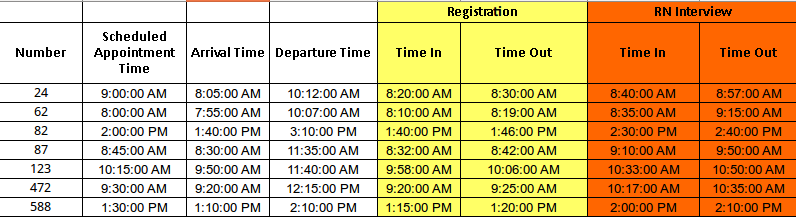
\includegraphics[scale=0.5]{sample1.png}

\quad

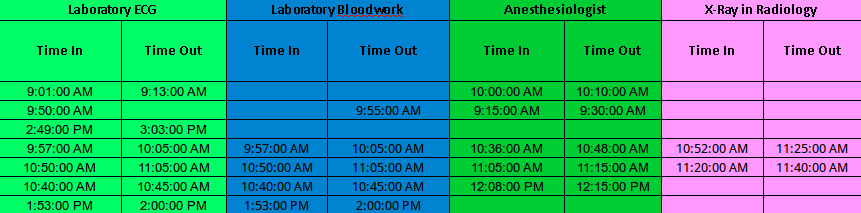
\includegraphics[scale=0.5]{sample2.png}

\newpage
\section{Schedule}

\begin{center}
\begin{longtable}{>{\raggedright\arraybackslash}p{0.1\textwidth}>{\raggedright\arraybackslash}p{0.15\textwidth}>{\raggedright\arraybackslash}p{0.55\textwidth}
>{\raggedright\arraybackslash}p{0.1\textwidth}
}

\caption{Testing Schedule}\label{Table_Schedule}\\\toprule

\bf Date Finished & \bf Test Type & \bf Event & \bf Testers\\\toprule

2016-11-20 & Intial Tests & Proof of Concept Demonstration & Development Team \\\midrule
2017-02-12 & Unit Tests & Demonstration Revision 0 & Developement Team \\\midrule
2017-02-12 & System Tests & Demonstration Revision 0 & Developement Team \\\midrule
2017-03-22 & Unit Tests & Test Report Revision 0 & Developement Team \\\midrule
2017-03-22 & System Tests & Test Report Revision 0 & Developement Team \\\midrule
2017-03-22 & Non-Functional Tests & Test Report Revision 0 & Developement Team \\\midrule
2017-04-04 & All Tests & Final Documentation & Developement Team \\\midrule

\bottomrule
\end{longtable}
\end{center}

\end{document}